\newcommand{\duedate}{3 October 2021}
\documentclass{16384_doc}
\newcommand{\assignmentname}{Assignment 4: IK, Trajectories, and Control}

\ifdef{\writeup}{\printanswers}

\begin{document}
\maketitle

\tableofcontents

\section{Overview}
This assignment reinforces the following topics:
\begin{itemize}

\item Analytic IK
\item Numerical IK
\item Trajectories for Robot Control

\end{itemize}

\section{Background}

\subsection{Analytical IK}

One approach to IK is to solve for joint angles given a workspace end effector
position manually, via algebraic methods or geometric
analysis, for each different type of manipulator.  This is very different from
FK, which is pretty much formulaic, going through the transforms of each
link to get the end effector position.  The range of arms for which analytical
solutions exist are only arms that are fully constrained, and solutions generally
have to be further manually inspected to check for an arm exceeding joint limits
or other practical considerations.

Analytical IK has the advantage that it is precise, fast (once you figure out
the solution), and global, meaning that you can always find a solution for joint
angles given an end effector position that is within the arm’s workspace.  So in
short, with analytical IK:
\begin{itemize}
\item If there is a solution(s), you will find it.
\item If there is no solution, you will know that.
\end{itemize}

A more flexible method we will discuss below is numerical IK, which can work
around most of the limitations posed by things like redundancy and joint limits.
However, it is approximate and local, meaning that you are not always guaranteed
to find a `good' solution.


\subsection{Numerical IK}

An alternative approach to analytical IK is numerical IK, or optimization-based
IK.  In this case we use the forward kinematics and a cost function to try to
find a solution to the inverse kinematics.  The general idea is to design a
function that takes in a desired end effector pose and produces a scalar `cost'
(often an error based on distance to the desired pose) that an optimizer will
try to minimize by varying the input variables. In this case the input variables
are joint angles which are used to calculate the forward kinematics as part of
the cost function.

Overall the process works like:
\begin{enumerate}
\item Pick a desired end effector pose
\item Pick an initial arm configuration (this is important detail; usually you
are already in a configuration that you wish to start from)
\item Evaluate the forward kinematics at the current configuration
\item Evaluate the update rule for the input variables (e.g., gradient descent,
a method based on the gradient of the cost function)
\item Check for `stopping conditions', often based on the change in cost or the
number of iterations (e.g., for gradient descent this can be related to the
magnitude of the gradient); if we meet these stopping conditions, then return
the current value of the input variables as our solution
\item Update the input variables and go back to step 3
\end{enumerate}

Different optimizers have different methods of picking the next configuration
to try, but most are based on gradient methods.  Essentially, they try to figure
out the slope of the cost function and trying to go ‘downhill’ until they reach a minimum.

There are distinct advantages and disadvantages of numerical IK compared to
analytical IK.

\subsubsection{Advantages}

\begin{itemize}
\item Numerical IK is a ‘black box’.  As long as you have forward kinematics for
an arm, you can make a cost function, pick an optimizer, and solve the inverse
kinematics.  It's general and relatively straightforward to implement.
\item Numerical IK can handle arms that are under-constrained (redundant) or
over-constrained.
\item You can modify the cost function for numerical IK to include whatever you
want.  Joint limits, knowledge of obstacles, other high-level requirements, etc.
can all be added relatively easily.
\end{itemize}

\subsubsection{Disadvantages}
\begin{itemize}
\item Numerical IK is a ‘black box’.  You do not necessarily get any intuition
into the underlying structure of the problem.  There might be multiple solutions
to a desired pose, or none at all.  You have to be careful with how you
interpret and use the result that an optimizer spits out.
\item Solutions are local, and subject to initial conditions.  Optimizers all
need an initial guess on where to start, and this guess can dramatically affect
the solution the optimizer finds.  The most reliable way to use numerical IK for
arms is to start in a configuration that is as close as possible to the desired
configuration, essentially ‘warm-starting’ the optimizer instead of searching
over large areas of the configuration space.
\item Numerical IK is usually less efficient computationally than analytical IK.
Frequently this is not the limiting factor for controlling a robot.  However,
there are some cases where you might want to sample the workspace a huge number
of times (one example of this in robotics research is the \emph{RRT}, or Rapidly
exploring Random Tree) and in such cases the speed of your IK might be the
limiting factor.
\end{itemize}

\subsection{Trajectories}

When controlling a robotic arm, it is usually important to handle things in a
way that is more sophisticated than just `banging' the arm from one
configuration to another.  The general idea is to not command anything a robot
 physically do.  Although we have not yet discussed dynamics in the class,
dynamics affect the ability to control the position or velocity of any
manipulator in the physical world.  In short:
\begin{itemize}
\item Real robots have mass, $m$
\item $F = ma$
\item $F$ is limited, so we should be careful about our desired $a$.
\end{itemize}

One way to mitigate effects of the dynamic limits of an arm is to use
\emph{trajectories} to smoothly move the arm from one configuration to another.
(When thinking about trajectories, you can pose them as trajectories in work
space or configurations space.  Here we'll just think of trajectories in
configuration space, but in the code problems you'll work with workspace
trajectories as well.)

\subsubsection{Bang-Bang Control (No Trajectories)}
The simplest method is to ignore the pesky bounds of reality and rely on the
underlying controller of the robot's actuators to `catch up' to your commands.
Depending on the specific application, and they way the low-level controllers
are tuned, this can actually work.  However, it has the disadvantage that the
robot's motion is less predictable since the low-level controllers dictate the
details of how the robot actually moves between the start and goal position --
which is something that you often want to have control over!  Additionally, with
this approach you are usually ‘jerking’ the arm aggressively which can be
dangerous and put unnecessary wear and tear on the arm’s joints.

\subsubsection{Constant Velocity (Better Than Nothing)}
The next-simplest method you might think of would be to respect the reality that a
robot’s joints can’t move with infinite speed.  Looking at the case of moving a
single DOF between two angles, we can choose an amount of time to take to move
between the angles and command a corresponding constant velocity.

$T_{\text{move}} = (\theta_{\text{end}} - \theta_{\text{start}}) / V_{\text{cruise}}$

This is a step in the right direction, but it has issues where we start and
stop.  To see the problem, let’s think about the position, velocity, and
acceleration.

\begin{center}
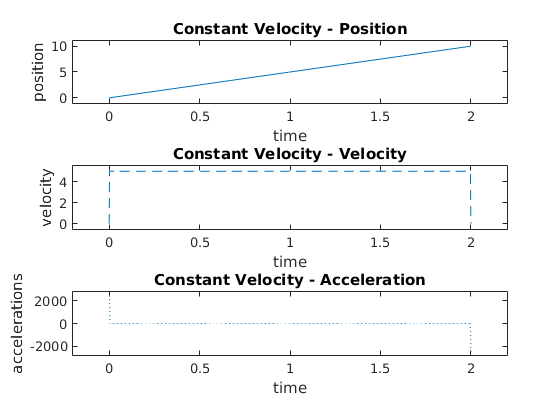
\includegraphics[scale=0.6]{generated_figures/constant_velocity.png}
\end{center}

Because we jump from stop to a constant velocity and back again, at the ending steps
we see big spikes in acceleration.  In theory, these spikes are infinite
acceleration, and in practice we will see some large finite value depending on
how finely we discretize time (size of our $\Delta t$ in the simulation or arm
controller).  Large accelerations are undesirable because if the arm has any
mass, then we are commanding large torques that are usually outside the
capabilities of the robot.  Again, the goal of using trajectories is to always
command things the arm can physically do, so that it is playing `catch up' as
little as possible.
    

\writtenSection

% \section{Written Questions}
% For all of the following questions, please fully compute all answers and show
% your work for full credit, unless otherwise specified. Submit your answers in a
% PDF entitled \verb!writeup.pdf! in your handin directory.  All answers must be
% typed, but diagrams may be hand-drawn and scanned in.  However, they must be
% tidy and fully legible! Consider drawing them in a black or blue pen.  All units
% are in radians and meters, where appropriate.

\begin{questions}

    \titledquestion{Analytical IK: PR robot}
    Given the PR Arm illustrated below from HW1.

    \begin{center}
        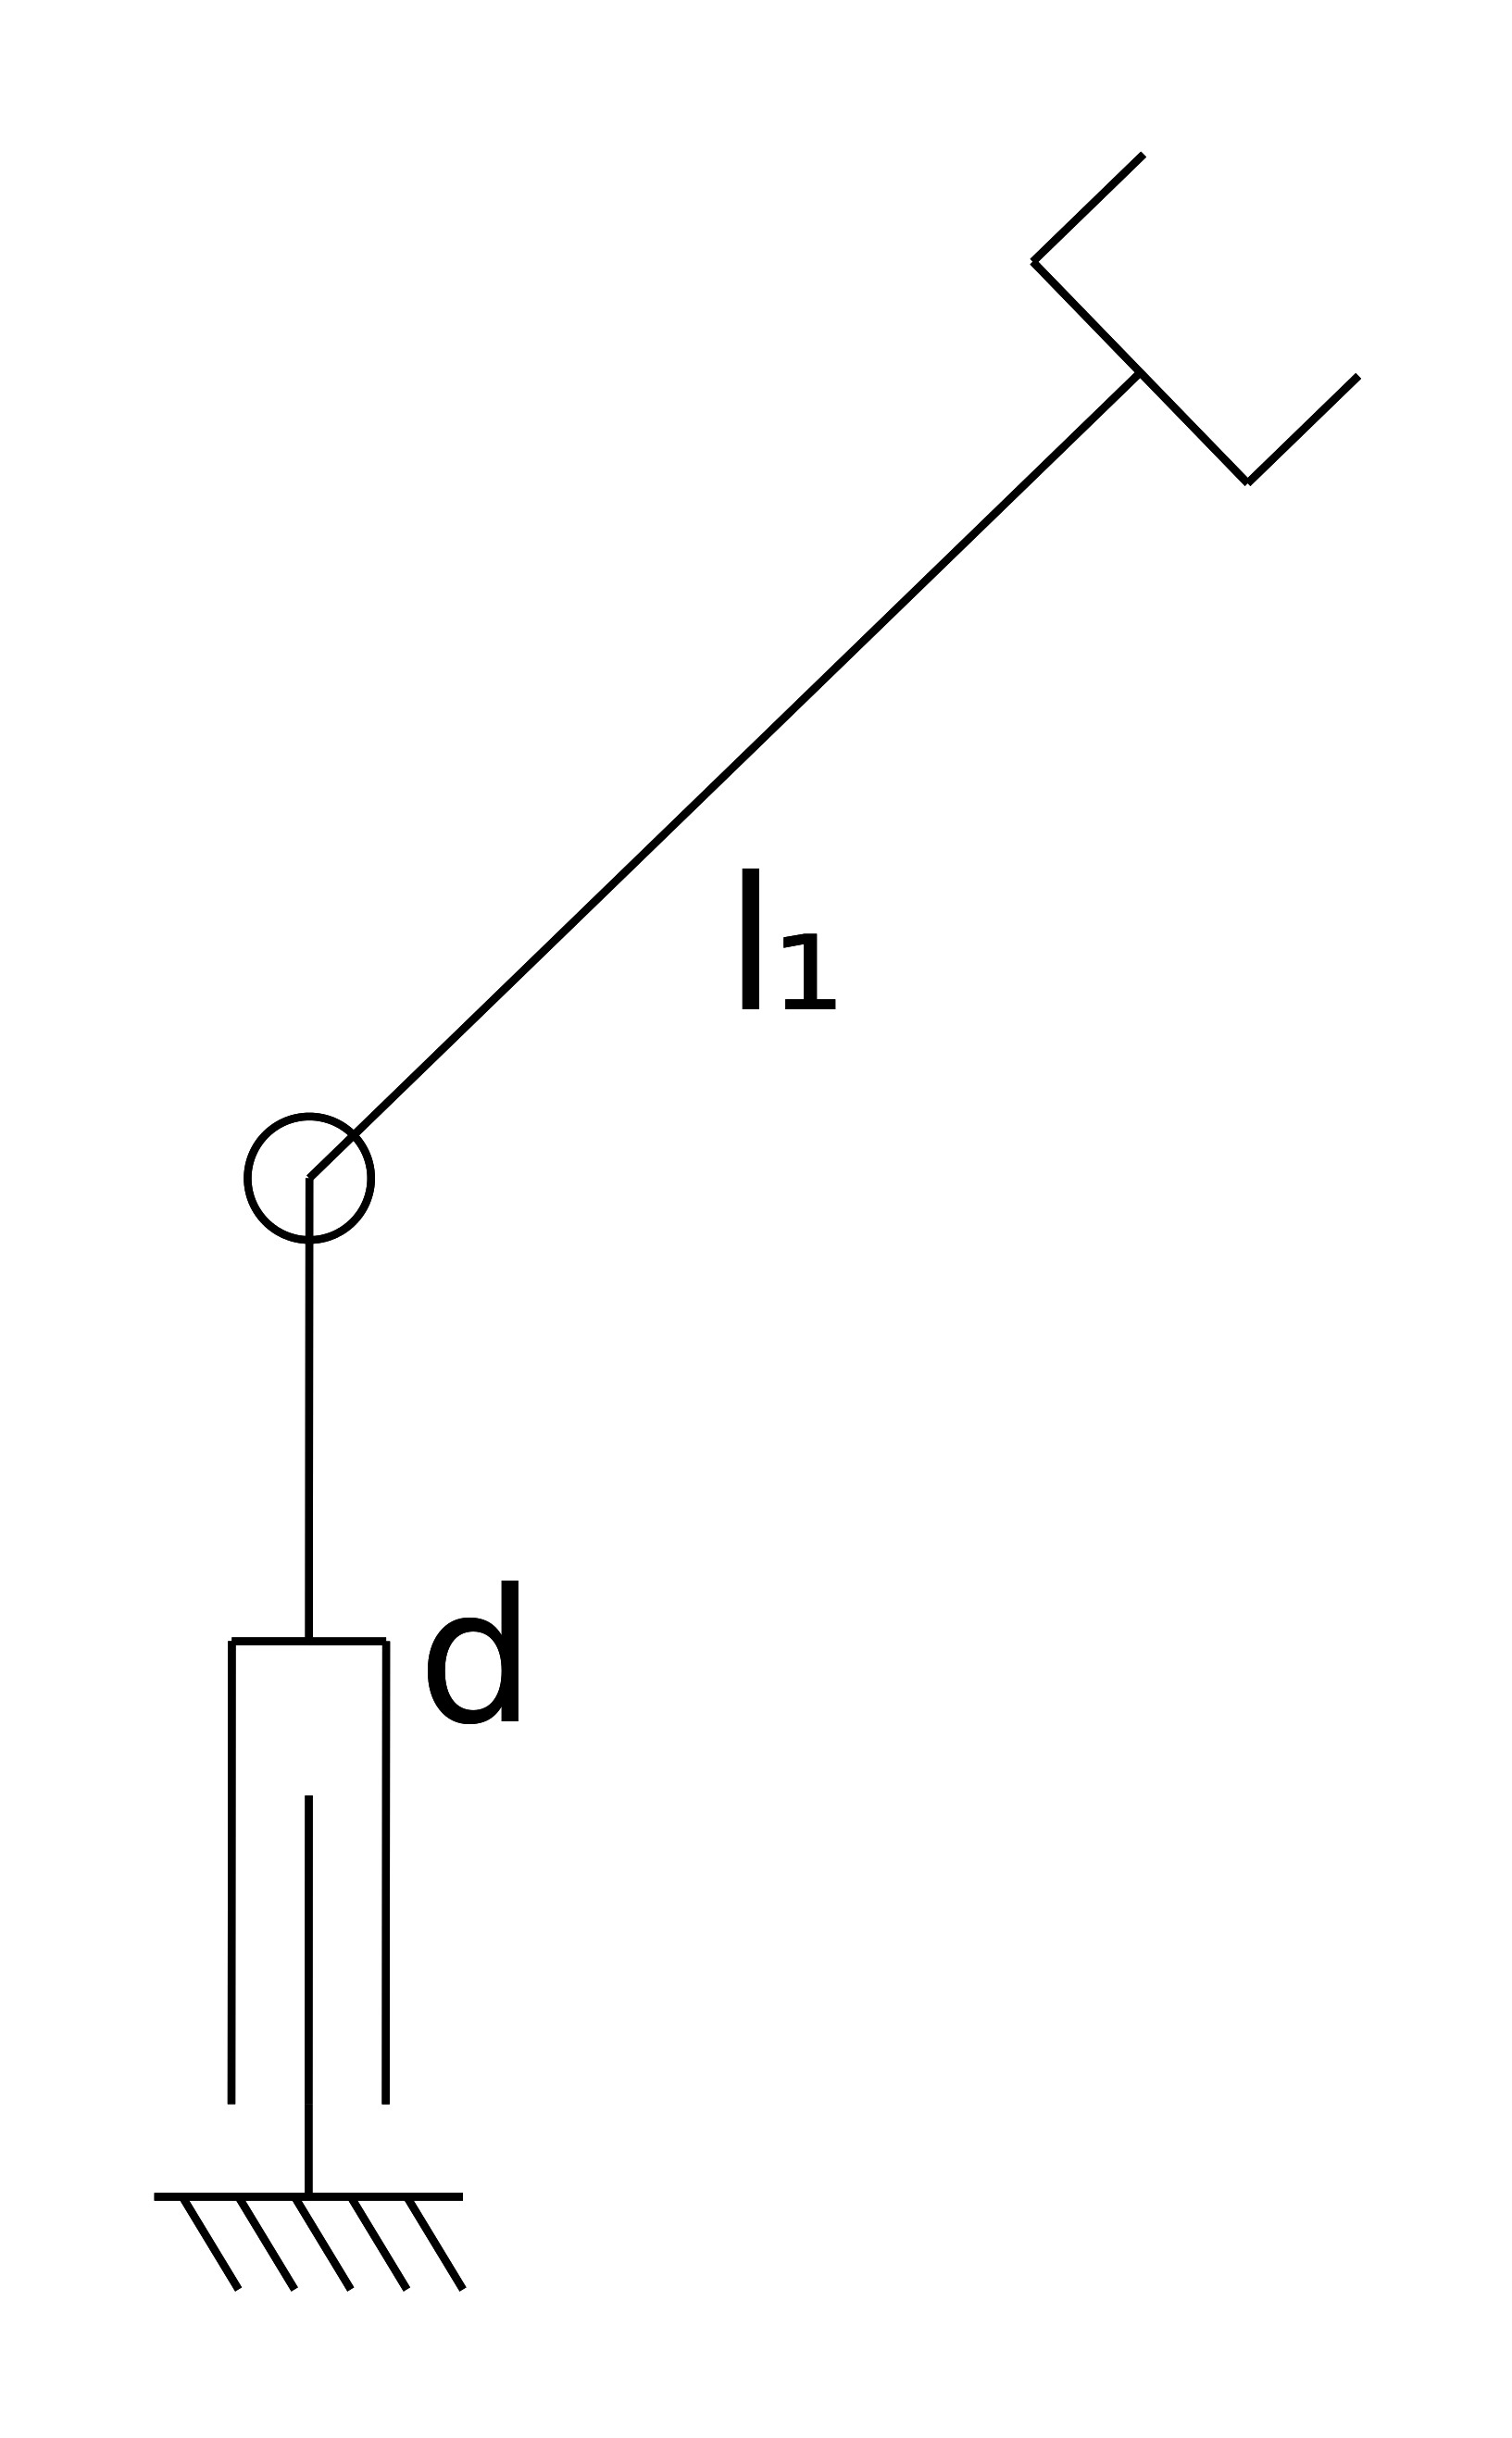
\includegraphics[width=1.5in]{generated_figures/robot_7.png}
    \end{center}

    \begin{enumerate} [label=\alph*.]
        \item \text{[15 points]} Analytically solve for $d$ and \th, which result
        in an end-effector pose of $\smcolvec{x_e\\y_e\\}$. % TODO: add frames to drawing
        
        \begin{tcolorbox}[height=3cm]
            % TODO: ENTER YOUR ANSWER HERE
        \end{tcolorbox}

    
        \item \text{[5 points]} Assume prismatic joint $d$ can go from 0 and 1 and $l_1$ is 1. Using your analytic IK from above, solve for $d$ and $\theta$ that results in an end-effector position of $\smcolvec{0.25\\1.5\\}$.

        \begin{tcolorbox}[height=3cm]
            % TODO: ENTER YOUR ANSWER HERE
        \end{tcolorbox}

        
        \item \text{[5 points]} Assume prismatic joint $d$ can go from 0 and 1 and $l_1$ is 1. Using your analytic IK from above, solve for $d$ and $\theta$ that results in an end-effector position of $\smcolvec{0.25\\0.5\\}$.

        \begin{tcolorbox}[height=3cm]
            % TODO: ENTER YOUR ANSWER HERE
        \end{tcolorbox}

        
        \item \text{[5 points]} Assume prismatic joint $d$ can go from 0 and 1 and $l_1$ is 1. Using your analytic IK from above, solve for $d$ and $\theta$ that results in an end-effector position of $\smcolvec{-0.25\\-0.75\\}$.

        \begin{tcolorbox}[height=3cm]
            % TODO: ENTER YOUR ANSWER HERE
        \end{tcolorbox}

        
    \end{enumerate}

    \titledquestion{Analytic IK: RPR robot}
    Consider the following robot

    \begin{center}
    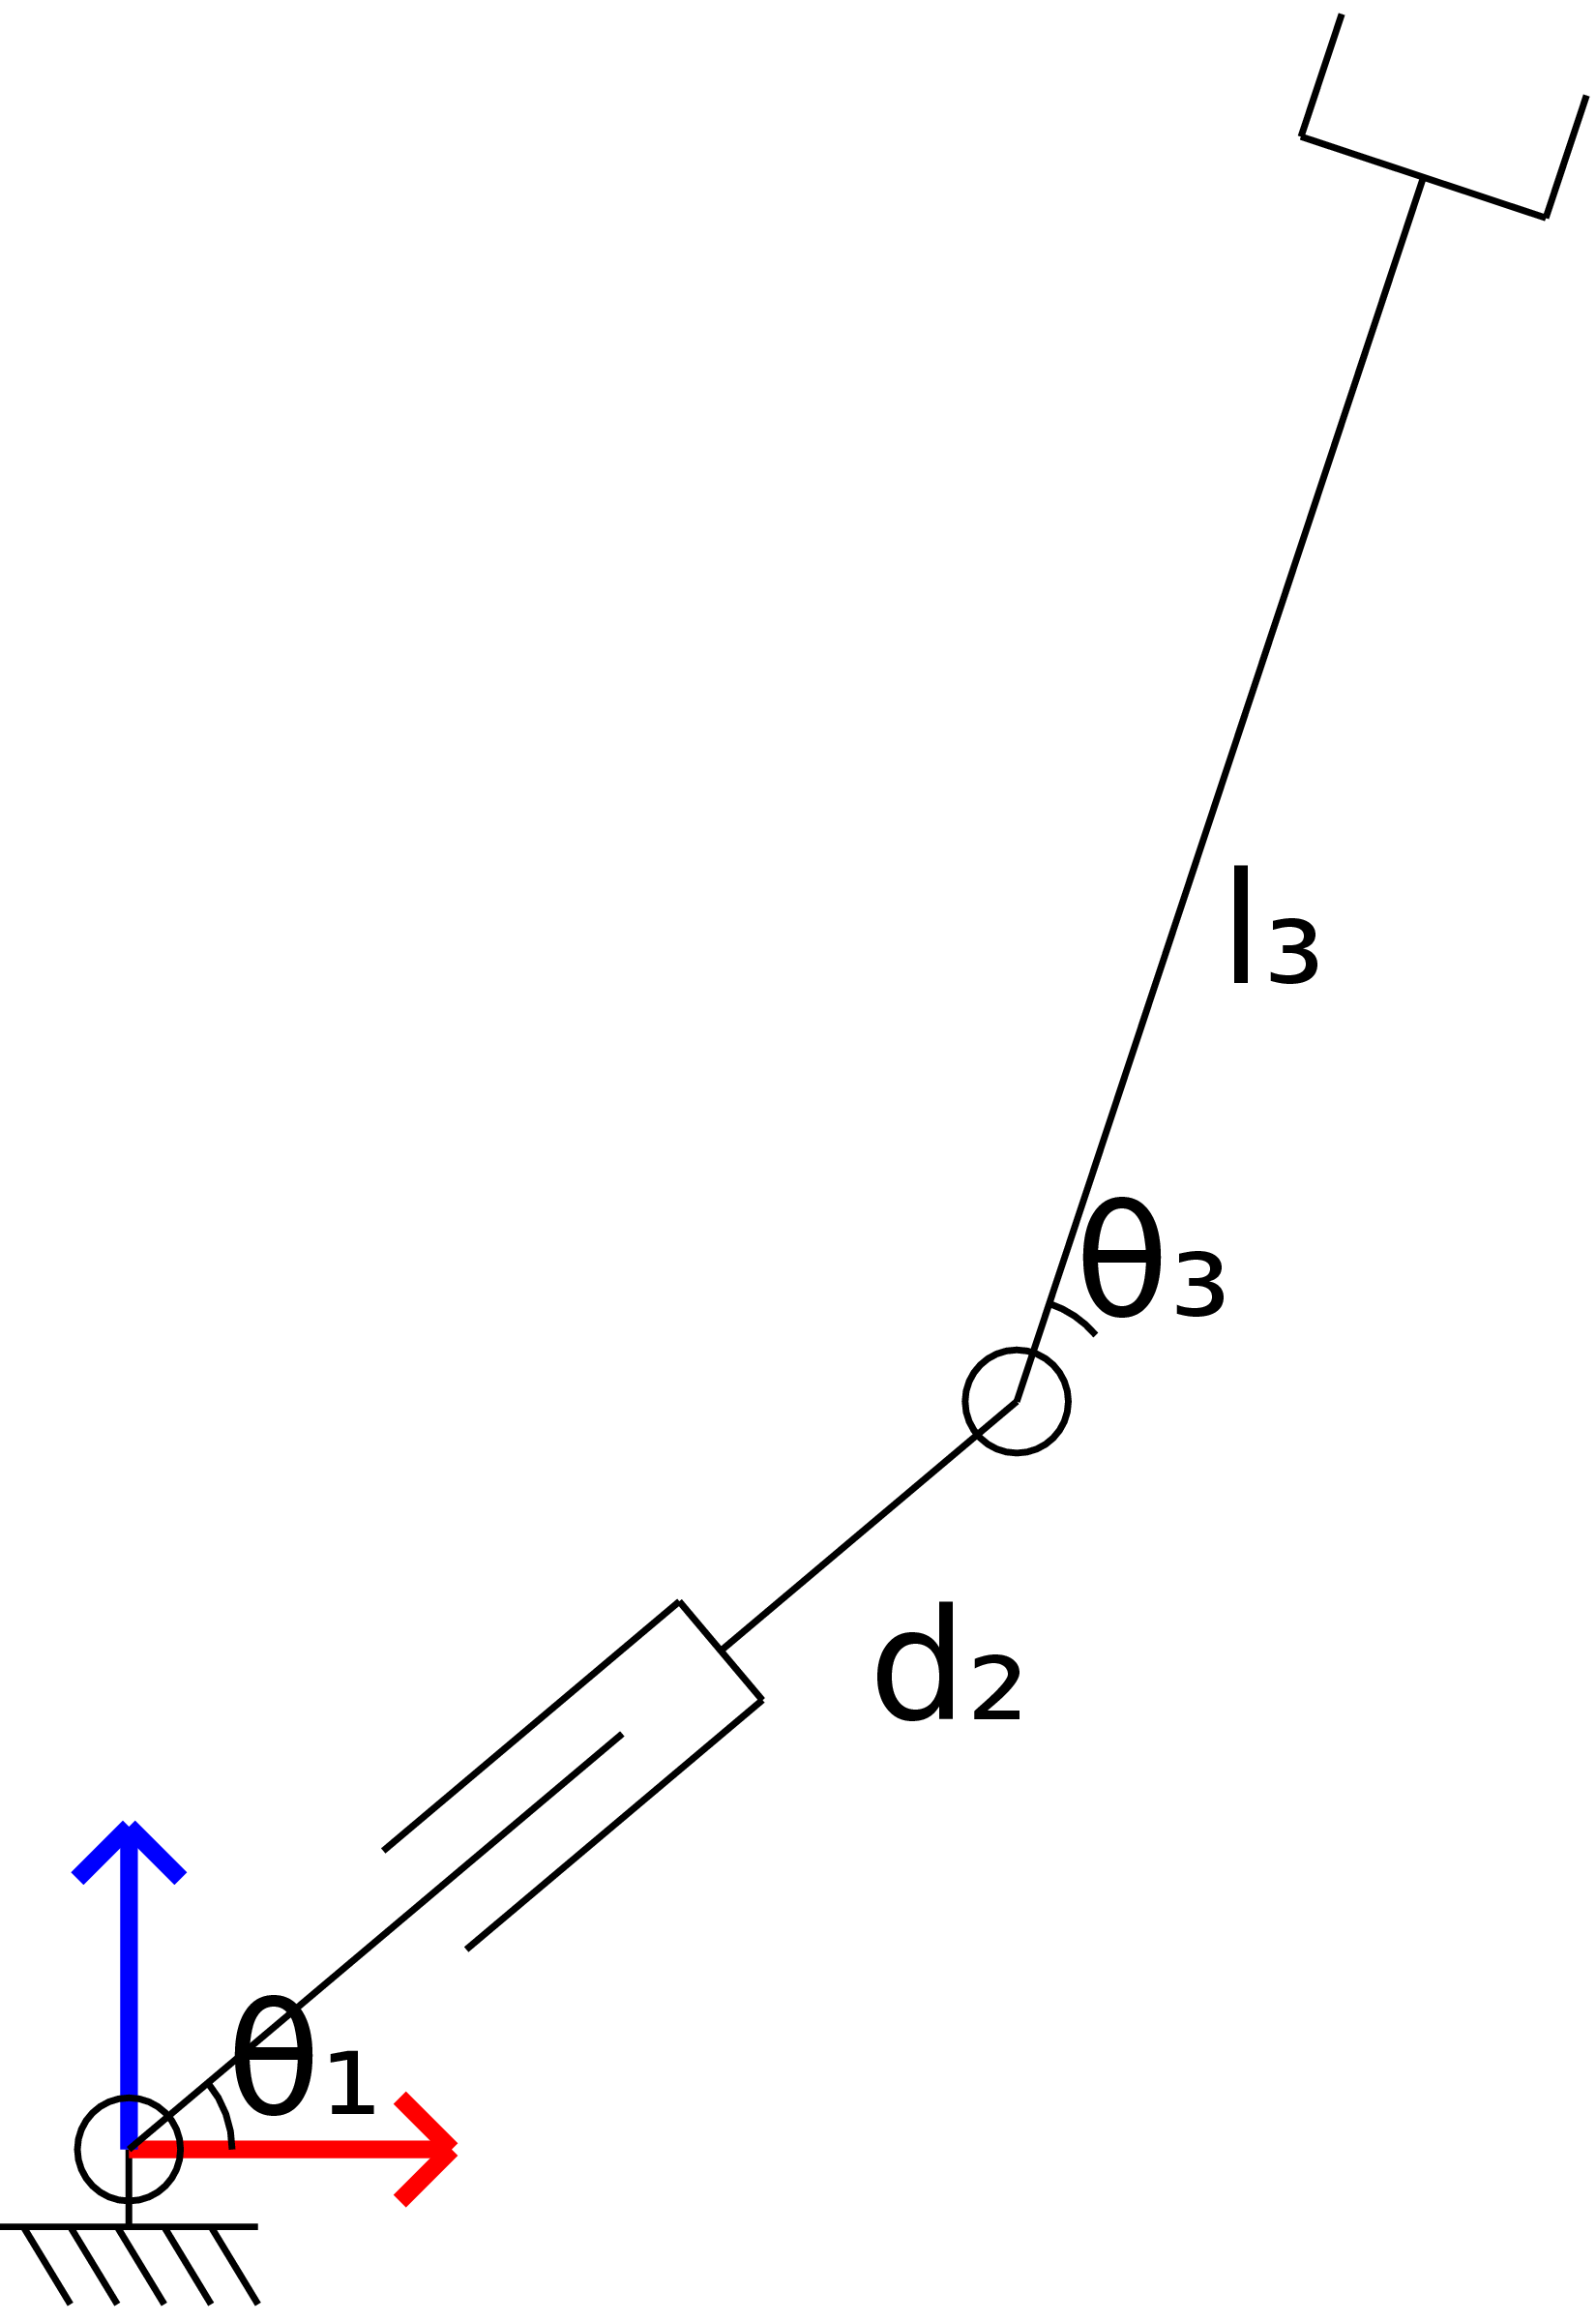
\includegraphics[scale=0.07]{generated_figures/rpr.png}
    \end{center}

    (Define the entire distance between the revolute joints as $d_2$).

    \begin{enumerate}[label=\alph*.]
        \item \text{[20 points]} Geometrically solve for \th[1], $d_2$, and \th[3] which result
        in an end-effector pose of $\smcolvec{x_e\\y_e\\\th[e]}$. Show your
        work! HINT: Break this problem down into an easier subproblem; are there
        known workspace positions of other parts of the robot, given the end
        effector pose?
        
        \begin{tcolorbox}[height=3cm]
            % TODO: ENTER YOUR ANSWER HERE
        \end{tcolorbox}

        
        \item \text{[10 points]} Assume there are no joint limits, except that $d_2 >= 0$. What
        (if any) limitations are there on achievable end-effector poses
        $\smcolvec{x_e\\y_e\\\th[e]}$.  Explain your answer in 1-2 sentences.
        
        \begin{tcolorbox}[height=3cm]
            % TODO: ENTER YOUR ANSWER HERE
        \end{tcolorbox}
        
    \end{enumerate}

    \titledquestion{Numerical IK: Cost function}
    Consider the following robot

    \begin{center}
    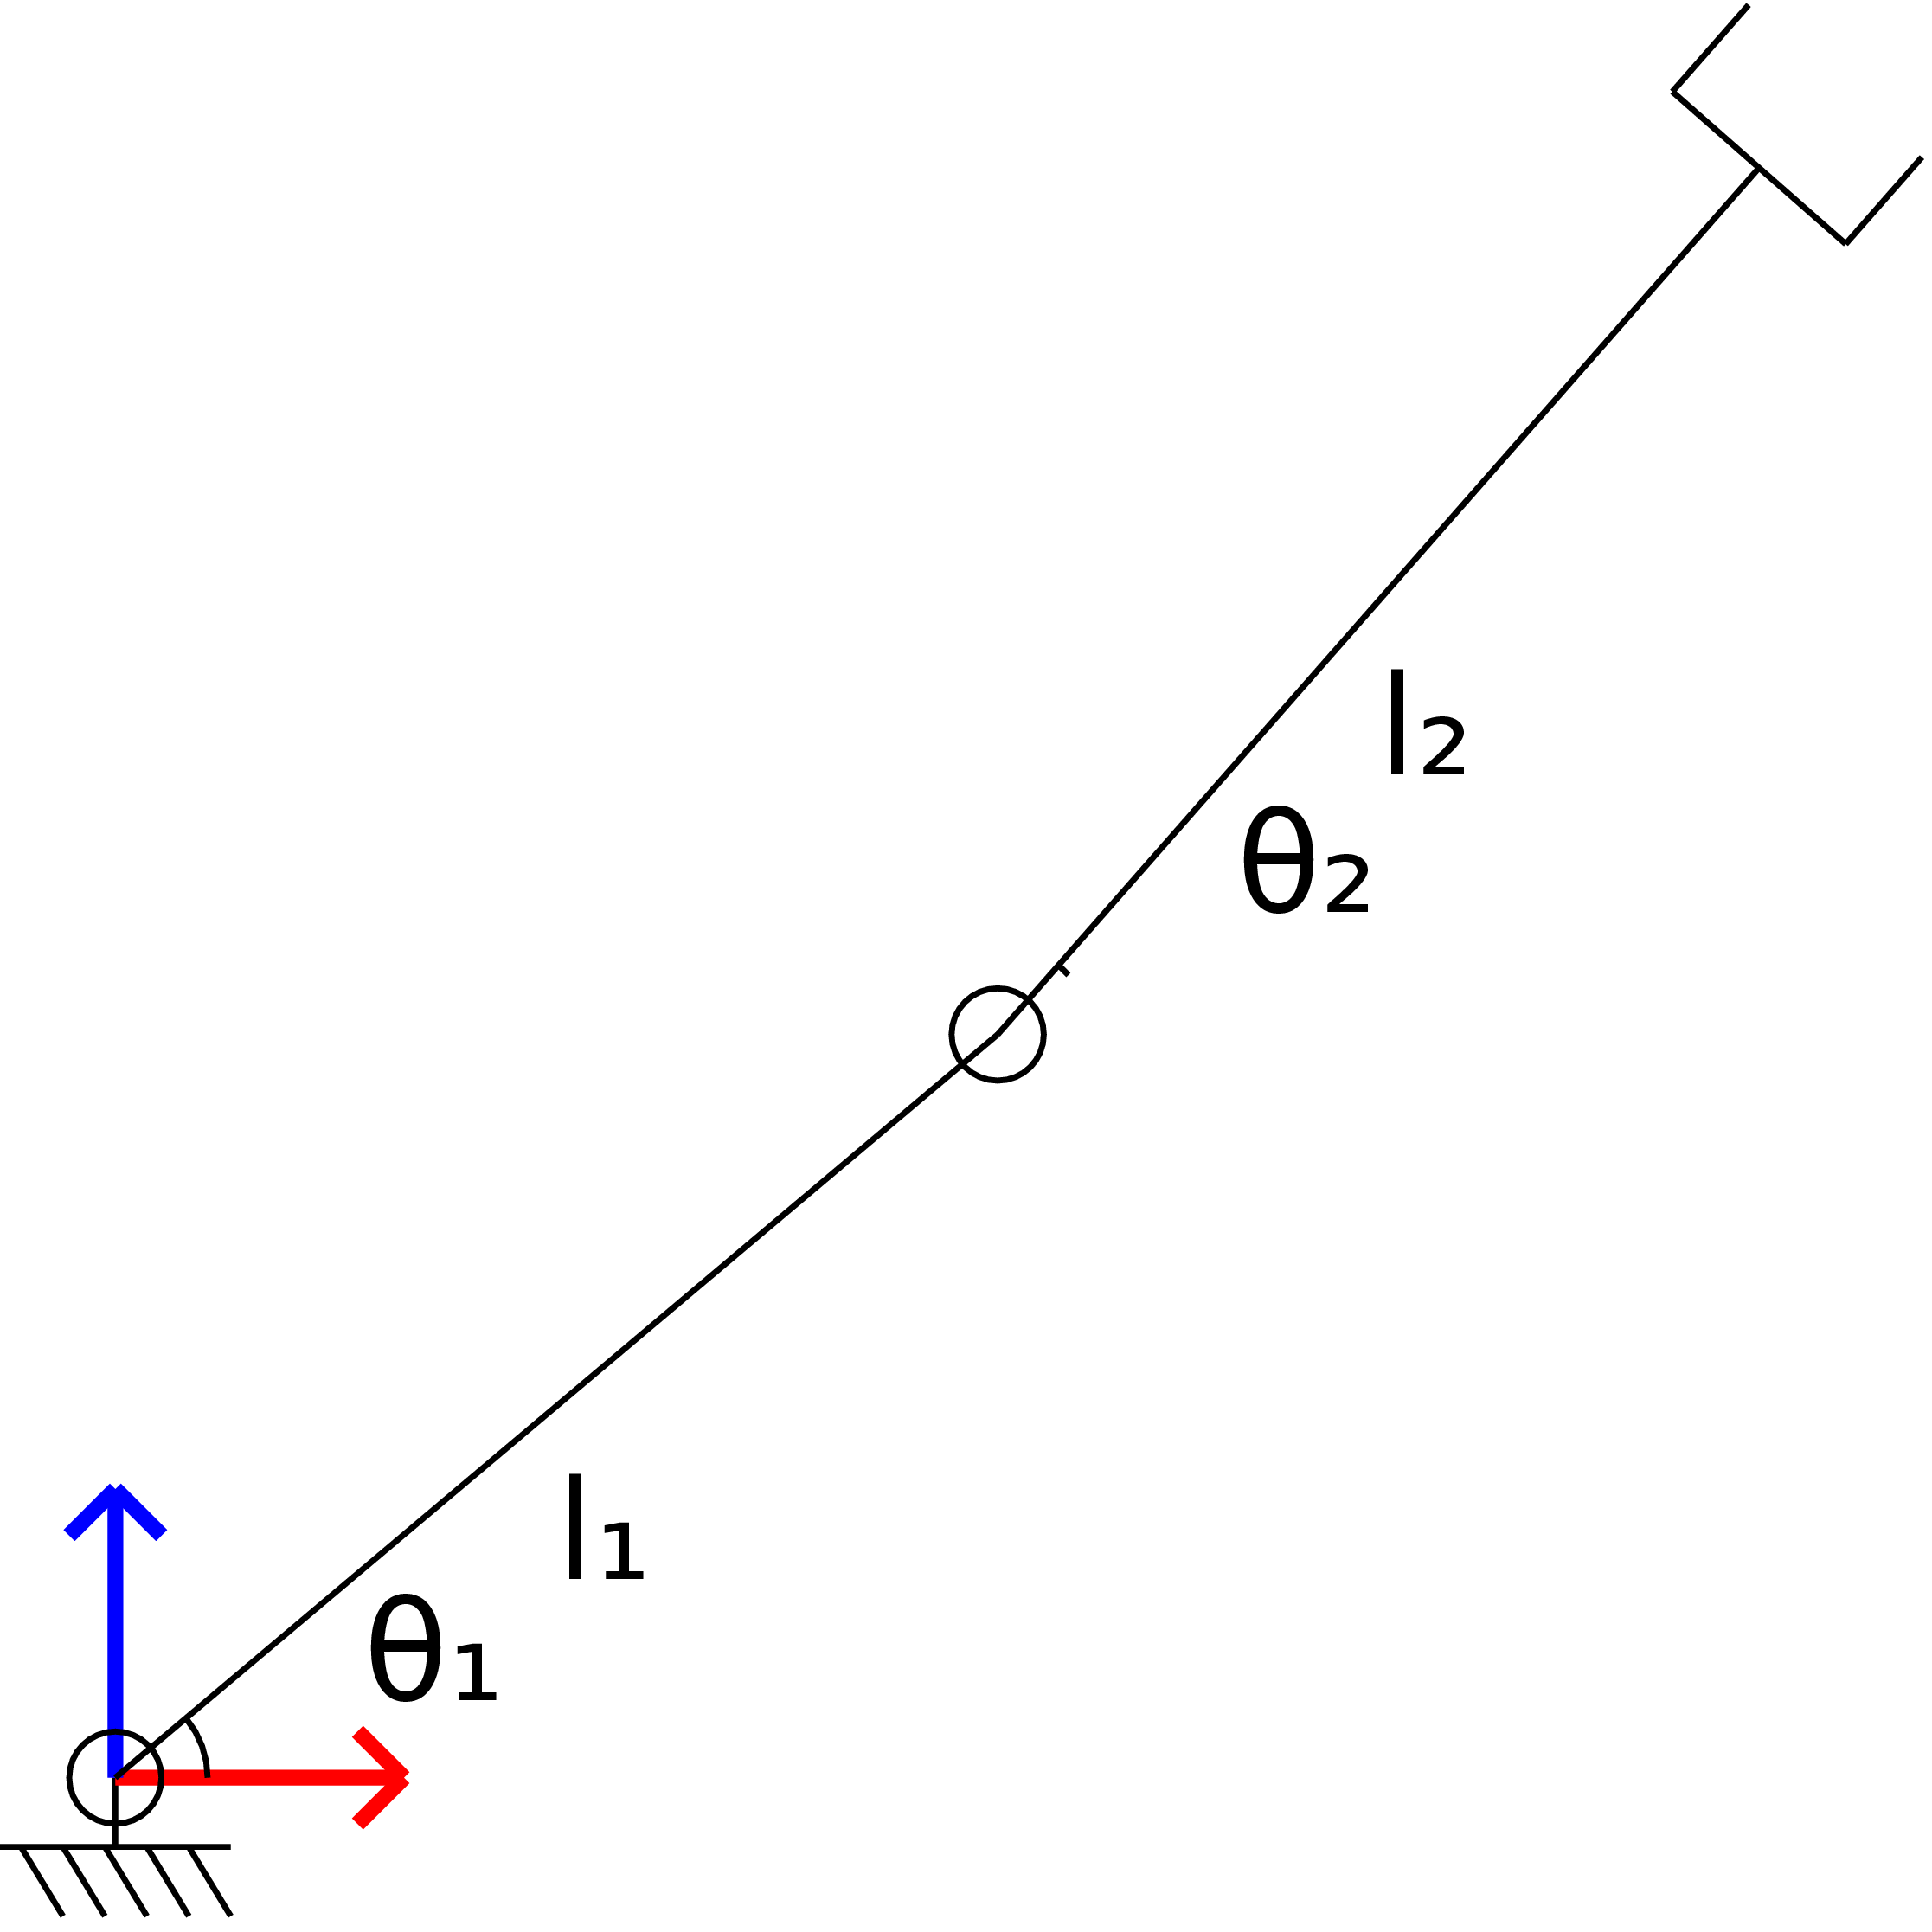
\includegraphics[scale=0.07]{generated_figures/rr.png}
    \end{center}

    \begin{enumerate} [label=\alph*.]
        \item \text{[10 points]} Let $p_e = \smcolvec{f_x(\th)\\f_y(\th)}$ (for forward kinematics $f$
        and joint configuration $\th$)  be the end effector position as a function of the configuration $\theta$. The goal is to find $\theta$ which achieves an end effector position as close as possible to the desired
        position $p_d=\smcolvec{x_d\\y_d}$. Let cost function $h$ be the square of
        the distance between $p_e$ and $p_d$. Write this cost function in terms
        of the forward kinematics function $f(\th)$ and $p_d$ (e.g. you may use $f_x$
        and $f_y$, but do not use $l_1$ or $l_2$).
        
        \begin{tcolorbox}[height=3cm]
            % TODO: ENTER YOUR ANSWER HERE
        \end{tcolorbox}

        \item \text{[10 points]} Write the gradient of $h$, $\nabla h(\th) = [ \partialfrac{h}{\th[1]}, \partialfrac{h}{\th[2]} ]^{T}$,
        in terms of $f$, $p$, and partial derivatives of $f$ with respect to
        $\th[i]$.  Note: do not actually write out the derivatives of $f$; just
        use, for example, $\partialfrac{f}{\th[1]}$. HINT: if you
        are not familiar with vector differentiation, first write out $h(\th)$
        as a scalar expression by multiplying the individual vectors, and
        then compute the required partial derivatives as given above in the
        definition of $\nabla h(\th)$.

        \begin{tcolorbox}[height=3cm]
            % TODO: ENTER YOUR ANSWER HERE
        \end{tcolorbox}

        \item \text{[10 points]} Reorder these terms to write this expression in terms of the
        end effector Jacobian, $J$, along with $f$ and $p$.
        
        \begin{tcolorbox}[height=3cm]
            % TODO: ENTER YOUR ANSWER HERE
        \end{tcolorbox}

        \item \text{[10 points]} What would the expression for the gradient from the previous part
        look like for a 100 link serial chain of revolute modules? Is there any
        difference?  Describe why or why not.
        
        \begin{tcolorbox}[height=3cm]
            % TODO: ENTER YOUR ANSWER HERE
        \end{tcolorbox}

    \end{enumerate}
    
    \newpage
\end{questions}


\section{Code Questions}

% File and function names below are \verb, which can't hyphenate; let TeX
% move them to the next line rather than run them into the margin.
\sloppy

In these problems you will extend the \verb!Robot! class from the last
assignment with Jacobians and inverse kinematics, use them to build
trajectories, and compute the torques that hold a real robot arm up against
gravity. Each part can also be run on a simulated xArm7, the arm used in the
lab.

\subsection*{Setup}

Copy the code handout to a location of your choice. Everything below is run
from the top level of that folder, the one containing
\verb!local_autograder.py!.

\textbf{If you have not installed it yet, or you end up getting package errors later on down the line, conside reinstalling the course's robot library.} The handout includes its own
copy of the library, in \verb!16384-robot-lib!. It carries the simulator, the
visualizer and the collision checker the demos use, and it may be newer than
the version you installed for an earlier assignment. Update your environment
from it:

\begin{verbatim}
    cd 16384-robot-lib
    conda env update -f environment.yml    # new machine: conda env create
    conda activate 16384
    cd ..
\end{verbatim}

This installs the library as the Python package \verb!xarm7_lib!, pointing at
the copy in your handout.

The four exercises live in their own directories:

\begin{itemize}
    \item \verb!ex1! --- forward kinematics, the numerical Jacobian, and two
        scripts that use it.
    \item \verb!ex2! --- numerical inverse kinematics.
    \item \verb!ex3! --- joint-space and workspace trajectories.
    \item \verb!ex4! --- gravity compensation for the xArm7.
\end{itemize}

\verb!ex1!, \verb!ex2! and \verb!ex3! each contain a copy of \verb!robot.py!.
Each exercise is graded with the copy in its own folder, so once a method works
in one, copy it into the others: \verb!ex2! needs your forward kinematics and
Jacobians, and \verb!ex3! needs both the work from \verb!ex1! and your inverse kinematics from \verb!ex2!.

\subsection*{Testing your work}

\verb!local_autograder.py! checks your functions against a set of stored test
cases. Run all of them, or one exercise at a time:

\begin{verbatim}
    python local_autograder.py               # everything
    python local_autograder.py -p ex1        # just ex1 (or ex2, ex3, ex4)
    python local_autograder.py --verbose     # list every failing case
\end{verbatim}

A failing run lists the first few cases that did not match, and why. The stored
cases live in \verb!exN/inK.txt! (inputs) and \verb!exN/outK.txt! (expected
outputs).

\textbf{A word of warning.} The autograder on Gradescope does not use those
stored outputs. It takes the same inputs, perturbs them by a small random
amount that is different on every submission, and compares your result against
a reference implementation. Code that reproduces the published numbers without
actually computing the answer will score zero there. Write the general solution
and the two graders will agree.

There is one deliberate difference between them. \verb!sample_velocities.py!,
\verb!jacobian_example.py! and \verb!linear_workspace_trajectory.py! all call a
\verb!Robot!. Locally they are given your own \verb!robot.py!, so they can only
pass once your \verb!Robot! does. On Gradescope they are given a correct
\verb!Robot!, so there they are graded on their own.

\subsection*{Seeing your code on the xArm7}

Every exercise has a demo that runs your code on a simulated UFACTORY xArm7:

\begin{verbatim}
    python local_autograder.py -p vis1    # ex1; vis2 to vis4 for the rest
\end{verbatim}

Each one opens a browser tab with sliders above a 3D view of the arm. Press
ctrl-c in the terminal to stop it. The demos work before you have written
anything: the arm still moves, and the terminal says which of your functions
isn't ready yet and why.

The xArm7 has seven revolute joints, and \verb!ex1!--\verb!ex3! are about planar
arms. The two are the same mechanism once four of the seven joints are held
still. The library's lab pose holds
\[
    \theta_2 = \piover{2}, \quad
    \theta_3 = \piover{2}, \quad
    \theta_5 = -\piover{2}, \quad
    \theta_6 = \piover{2},
\]
which leaves joints 1, 4 and 7 with their rotation axes all parallel to the
world $z$-axis. What can still move is then exactly a planar RRR arm: joint 1 at
the shoulder, joint 4 at the elbow, joint 7 at the wrist, with a drawn 10\,cm
tool as the third link. The demos measure the link lengths off the robot model
and build your \verb!Robot! with them, so your code is run on the real geometry
of the arm.

\begin{questions}
    \titledquestion{\text{[40 points]} Forward Kinematics and the Numerical Jacobian}

    Complete \verb!ex1/robot.py!, \verb!ex1/sample_velocities.py! and
    \verb!ex1/jacobian_example.py!.

    \begin{enumerate}  [label=\alph*.]
        \item \text{[15 points]} \textbf{Forward kinematics}

        Reimplement or copy your \verb!forward_kinematics! from the last assignment into the
        marked section of \verb!ex1/robot.py!. It returns a $3 \times 3 \times
        (n+1)$ array of homogeneous transforms. \verb!frames[:, :, i]! is the
        frame at the base of link $i$, already rotated by joint $i$, and
        \verb!frames[:, :, -1]! is the end effector, a translation along the last
        link with no further rotation.

        \item \text{[15 points]} \textbf{Numerical Jacobian: implementation}

        The next task is to write the last Jacobian you'll ever need: one that
        works for any frame generated by the forward kinematics. Fill in the
        \verb!jacobians! method in \verb!ex1/robot.py!.

        This function computes a $3 \times n$ Jacobian (where $n$ is the number of
        joints) for each of the $n+1$ frames, and returns them stacked as a
        $3 \times n \times (n+1)$ array. The code describes the conventions used
        for the arguments and result.

        Whereas in previous assignments you have calculated the analytic
        derivative for each element of the Jacobian, here you will use a
        numerical approach. Given a general function $g(x)$, one can approximate
        its derivative $g'(x)$ by the forward difference
        $(g(x+\epsilon) - g(x)) / \epsilon$, or more accurately by the central
        difference $(g(x+\epsilon) - g(x-\epsilon)) / (2\epsilon)$.

        In the code, we will take the same approach for each element of the
        Jacobian. For example, for the element corresponding to the $x$ value for
        frame $i$ and joint $j$ (given a joint configuration $\Q$), evaluate the
        forward kinematics $f_x$ at $\Q + \Delta \mathbf{q}_j$ (and, for a central
        difference, at $\Q - \Delta \mathbf{q}_j$), where $\Delta \mathbf{q}_j$
        is a vector of zeros with $\epsilon$ for element $j$, and divide the
        difference by $\epsilon$ (or $2\epsilon$). Use the $\epsilon = 0.001$
        given in the code; either difference is accepted. As with the analytical
        approach, the rotation row is filled in by inspection for now.

        \item \text{[5 points]} \textbf{Verification: sample velocities}

        Fill in \verb!compute_kinematics! in \verb!ex1/sample_velocities.py!. For
        every time step it computes the end effector position with the forward
        kinematics, and its velocity by multiplying the end effector Jacobian by
        the joint velocities. Then run the script:

\begin{verbatim}
    cd ex1
    python sample_velocities.py
    cd ..
\end{verbatim}

        Verify that:
        \begin{enumerate}[label=(\roman*)]
            \item On the first plot, the paths match \emph{and} the end effector
                velocity vectors are tangent to the path that it takes.
            \item On the second plot, the $x$ and $y$ velocities match.
        \end{enumerate}

        Also, use your \verb!jacobians! to find the Jacobian for an RRR arm at
        configuration $\smcolvec{0\\0\\0}$. Look at the third row of the Jacobian
        for each frame, the effect of joint angle velocity on the orientation of
        the frame. For the first frame (recall, attached to the first link), only
        the first joint angle should have an effect (i.e., this row should be
        $[1, 0, 0]$). For the second frame, the first and second joint angles
        should have an effect. The third and fourth frames (third link and end
        effector, respectively) should each be affected by the motion of every
        joint.

        \item \text{[5 points]} \textbf{Application: joint torques for a wrench}

        Because we have a Jacobian for any planar revolute-joint based arm, we
        can now address problems that would have been much more difficult
        before. Imagine a RRRRRRRRRR arm (10 R's), with links each equal to $5$.
        Using the \verb!Robot! class you have written, compute the joint torques
        necessary to apply a wrench\footnote{Recall this is a combined force and
        torque vector; the first and second terms are forces in $x$ and $y$, and
        the third term is a moment.} of $\smcolvec{0\\5\\2}$ with the end
        effector when the robot is at the following configuration:
        \[
        \mathbf{\Theta} = \smcolvec{0, 0.1, 0.2, 0.3, 0.4, 0, -0.1, -0.2, -0.3, -0.4}^T
        \]

        Fill in \verb!compute_joint_torques! in \verb!ex1/jacobian_example.py!:
        it takes a robot, its joint angles and a wrench, and returns
        $\Jt \mathbf{w}$ for the end effector Jacobian. Running the script
        (\verb!cd ex1; python jacobian_example.py!) builds the 10R arm above and
        prints the torques.

        (Just for fun, imagine the number of terms for the analytic Jacobian for
        this arm. If you could write that out the very first time without making
        a mistake or a sign error, you might be the first person to ever do
        so\ldots)

        \item \textbf{See it on the arm}

\begin{verbatim}
    python local_autograder.py -p vis1
\end{verbatim}

        The page has two rows of sliders. The \verb!theta! sliders set the three
        joint angles and the arm follows them. The \verb!dtheta! sliders set a
        joint velocity $\dot{\mathbf{\Theta}}$; the arm does not move with these,
        they only set the velocity the arrows below are drawn for.

        Over the arm, the demo draws:
        \begin{itemize}
            \item a yellow skeleton through the frame origins your
                \verb!forward_kinematics! returns, with an axis triad at your
                end effector frame. When your kinematics are right the skeleton
                lies inside the arm and the triad sits on the red tool tip.
            \item a \textbf{blue} arrow: your end effector velocity,
                $\J\,\dot{\mathbf{\Theta}}$, from your \verb!jacobians!.
            \item a \textbf{green} arrow: the tip velocity the arm actually has
                at that joint velocity, computed from the arm itself. When your
                Jacobian is right the blue arrow covers the green one.
        \end{itemize}

        The status line under the sliders gives the numbers: your tip position
        against the measured tip, and your velocity against the arm's. Try
        setting one \verb!dtheta! slider at a time and check that each arrow is
        perpendicular to the line from that joint to the tip.

    \end{enumerate}

    \titledquestion{\text{[25 points]} Numerical Inverse Kinematics (IK)}

    Complete \verb!ex2/robot.py!.

    \begin{enumerate} [label=\alph*.]

        \item \textbf{Implementation}

        The next extension to the \verb!Robot! class is a function to compute
        inverse kinematics using gradient descent, as discussed in lecture. Fill
        in the \verb!inverse_kinematics! method in \verb!ex2/robot.py! (after
        copying in your forward kinematics and Jacobians from \verb!ex1!).

        This function accepts a vector of joint angles for initial conditions and
        a desired end effector location. It returns the resulting joint angles
        that are the solution of the gradient descent process. The code describes
        the conventions used for the arguments and result, and gives the step
        size, stopping condition and iteration limit to use.

        For this problem, assume the cost function is the sum of squared errors
        between the end effector and the goal point, ignoring joint angle limits.
        Use the solution to the second written problem to help compute the
        gradient of the cost function, and use a loop to continue updating the
        joint angles until no significant progress is made. \textbf{REMINDER}:
        You use the \emph{negative} gradient in this process, multiplied by a
        small step size $\alpha$.

        Your code should handle two cases:
        \begin{itemize}
            \item If the goal is a $2 \times 1$ vector, it should only consider the
                $[x, y]^T$ position of the end effector.
            \item If the goal is a $3 \times 1$ vector, it should consider the
                $[x, y, \theta]^T$ pose of the end effector.
        \end{itemize}

        \textbf{HINT 1}: Note that the \verb!end_effector! method in the
        \verb!Robot! class returns the end effector's $[x, y, \theta]^T$ pose.
        This will be very useful in coding the equation!

        \textbf{HINT 2}: For the $3 \times 1$ goal vector case, note that the form
        of the solution does not change; you must simply use an additional
        component of the pose and update your calculations accordingly.

        \item \textbf{Verification}

        To verify the results, solve the examples illustrated in the following
        figures:

        \begin{center}
        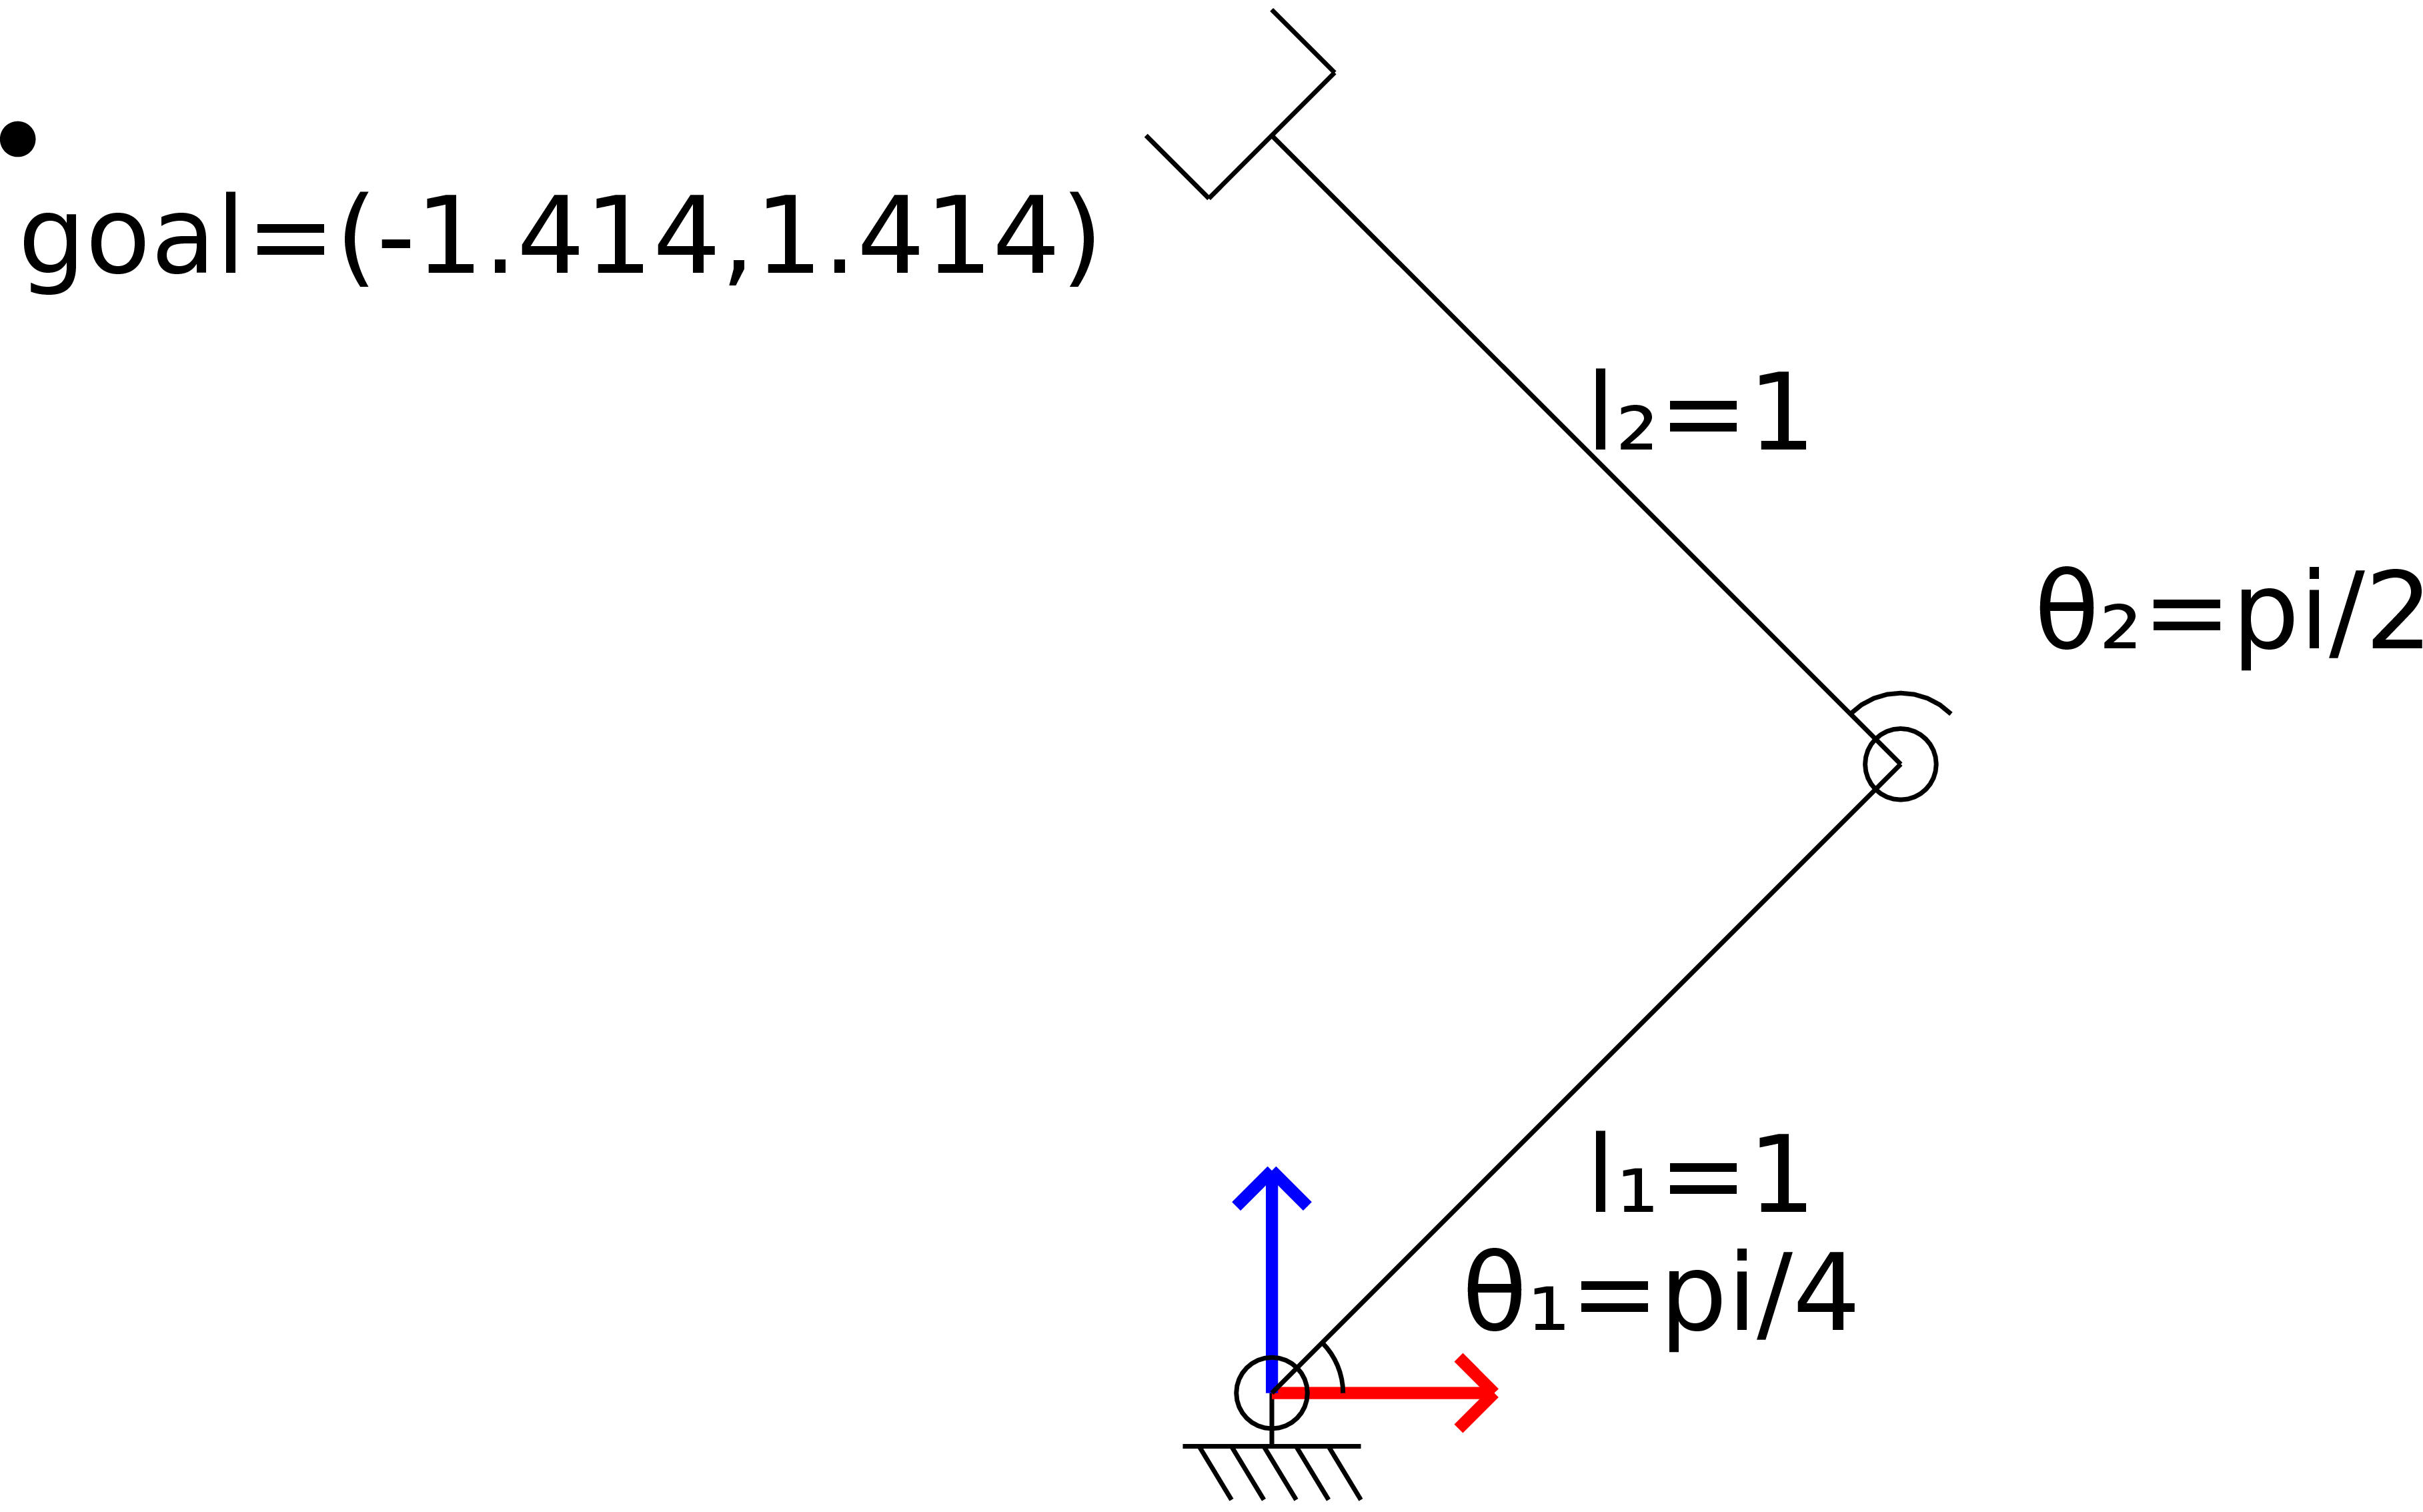
\includegraphics[scale=0.035]{generated_figures/ik1.png}
        \end{center}
        \begin{center}
        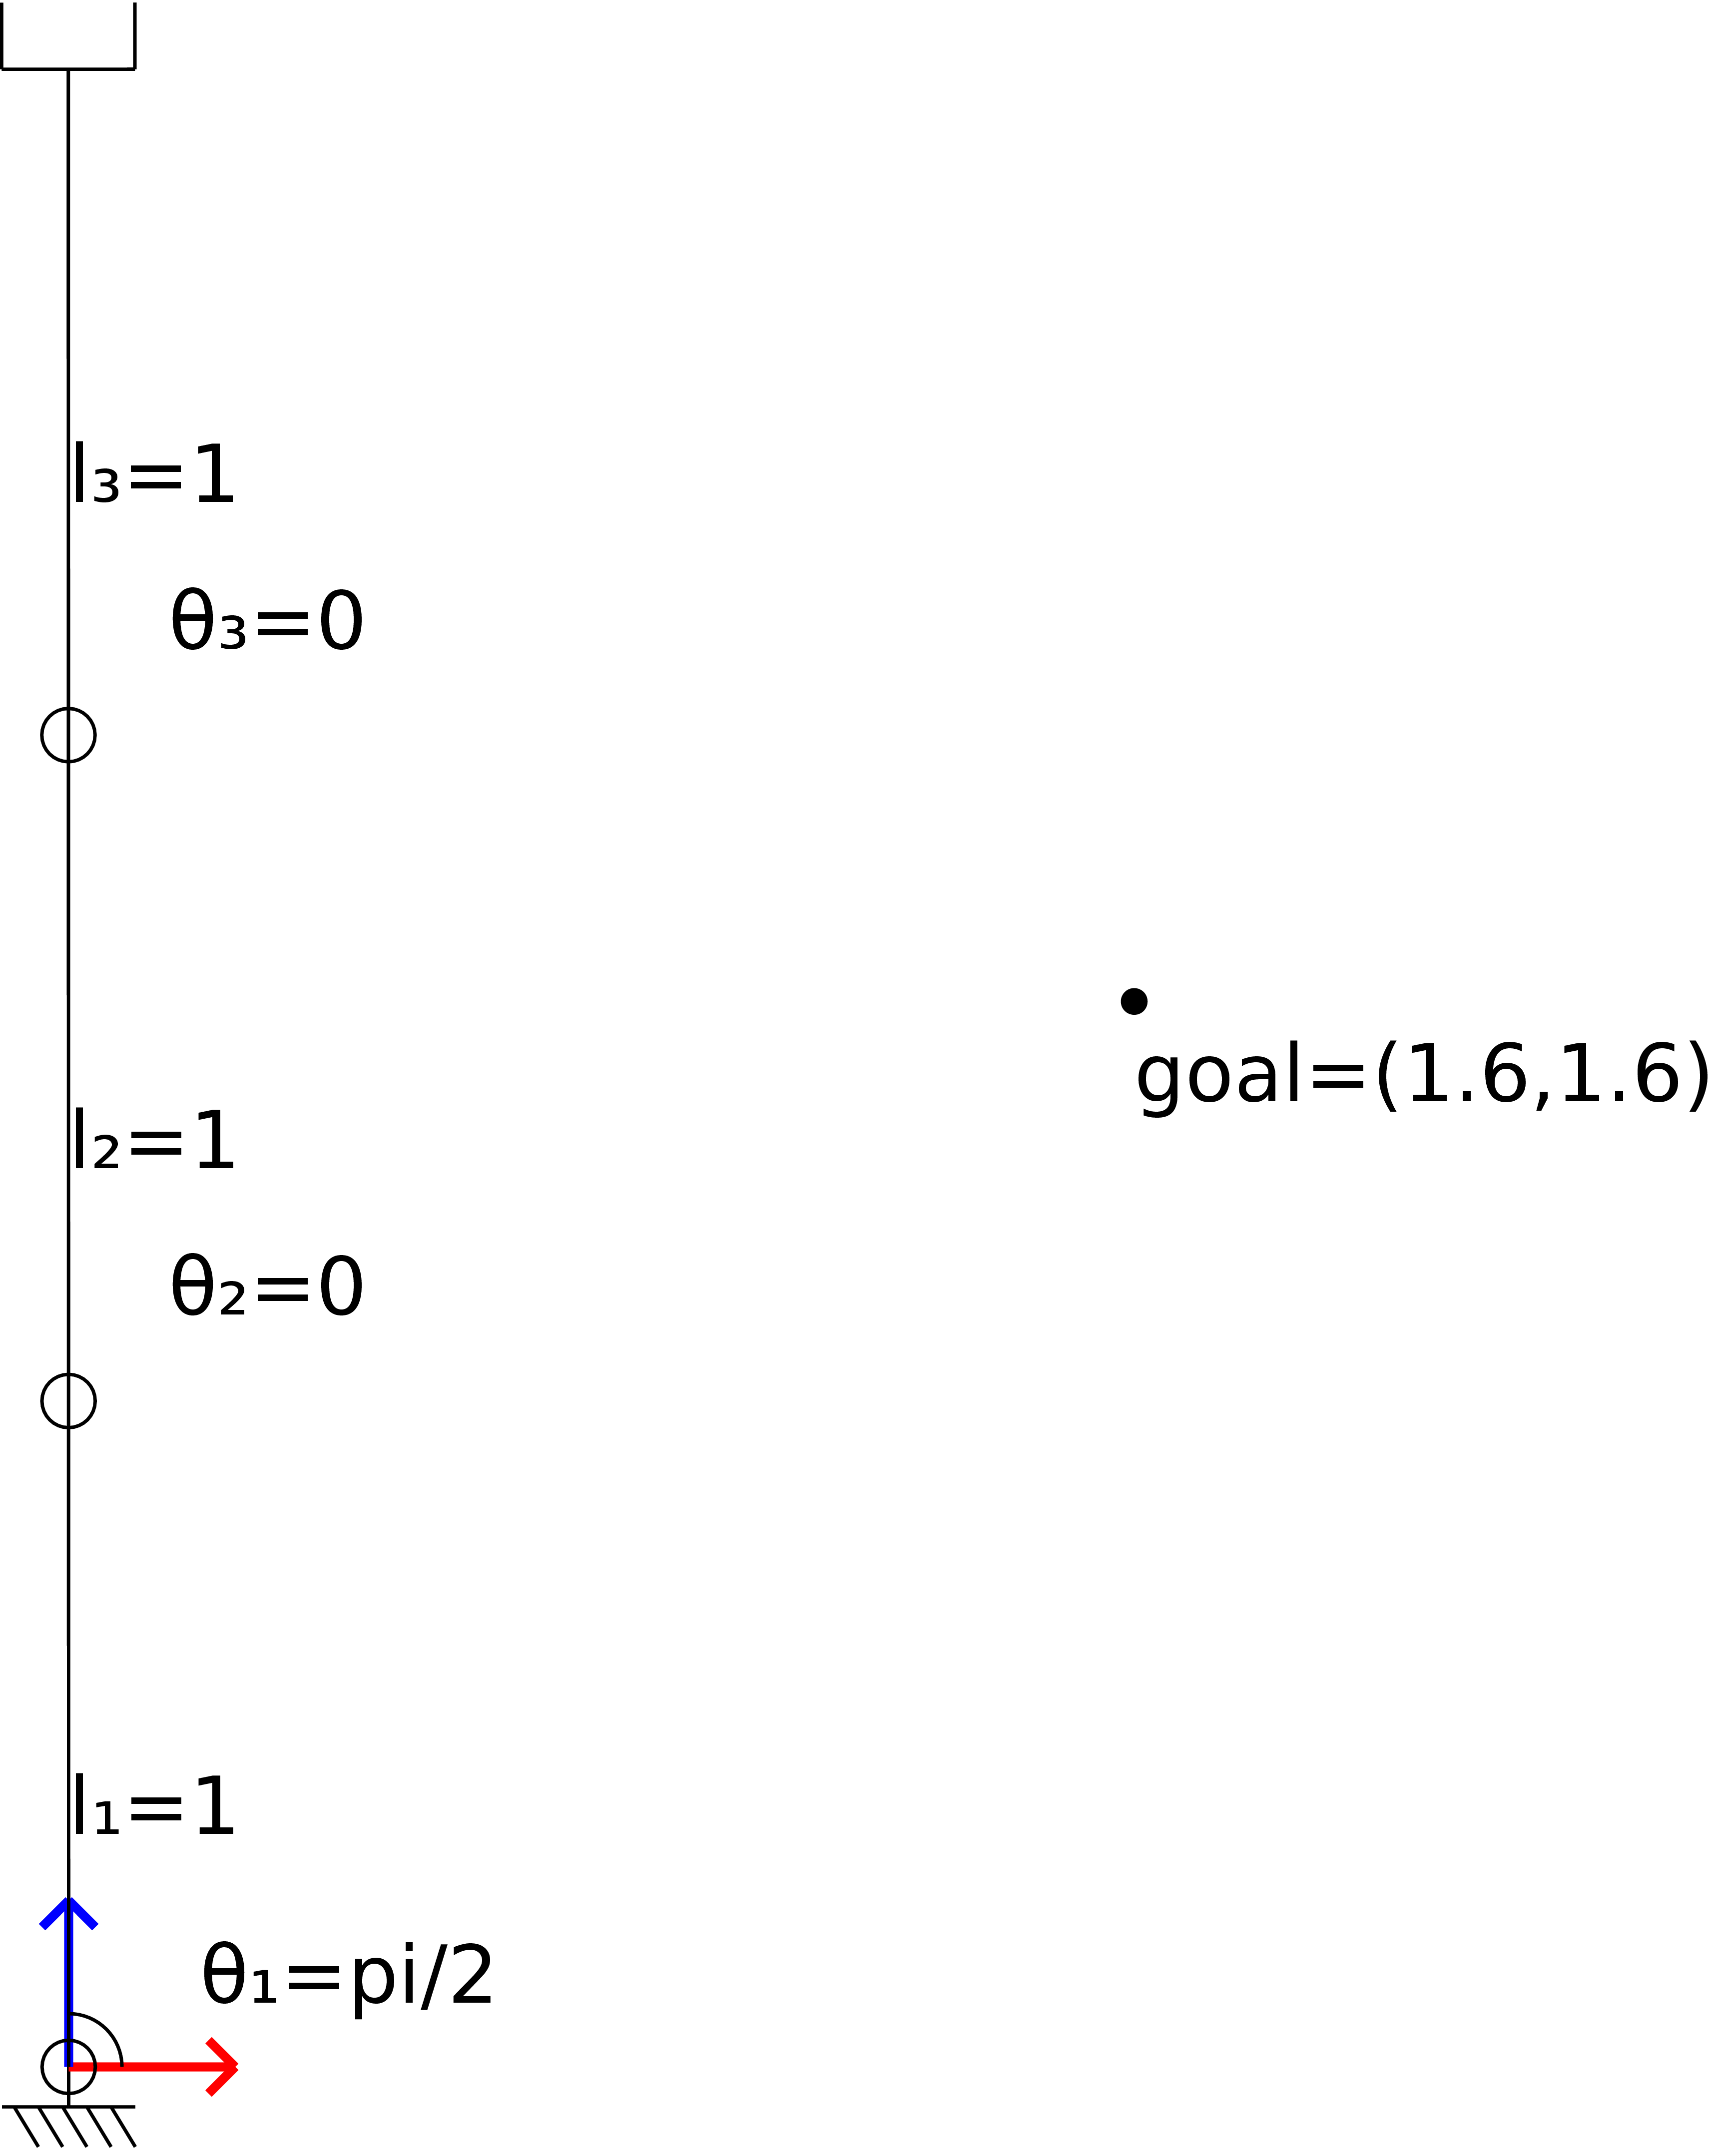
\includegraphics[scale=0.035]{generated_figures/ik2.png}
        \end{center}
        \begin{center}
        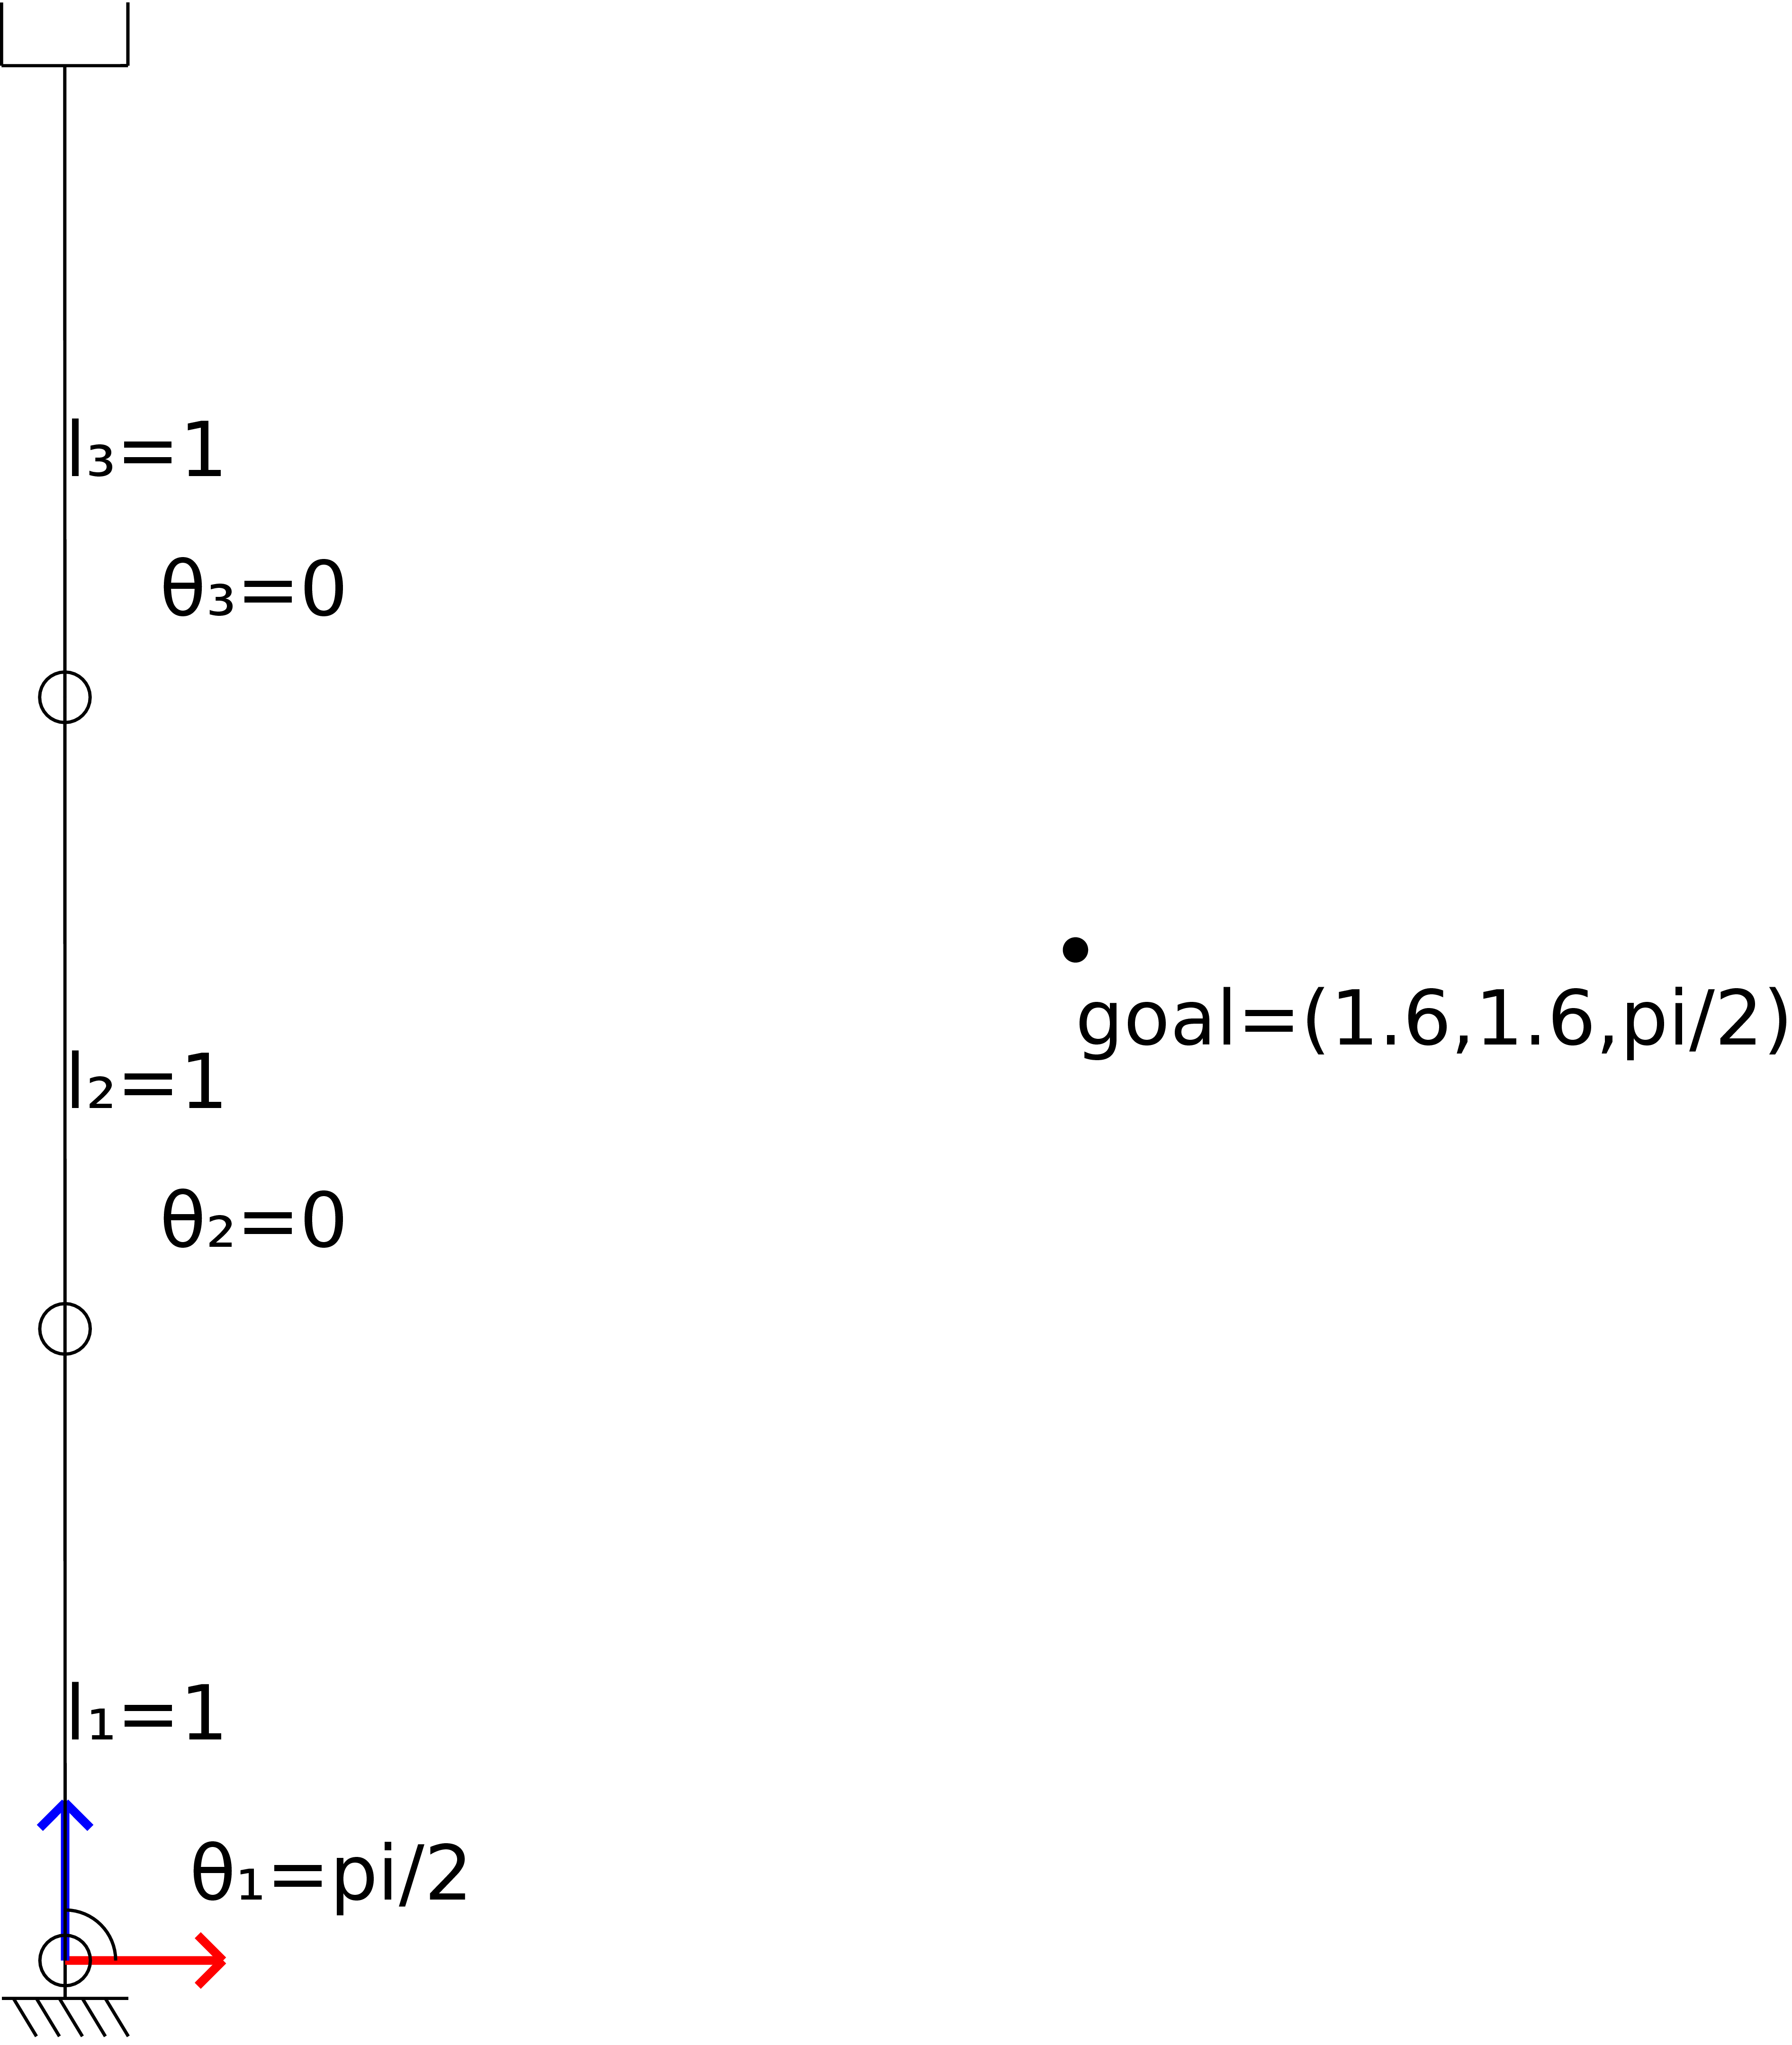
\includegraphics[scale=0.035]{generated_figures/ik3.png}
        \end{center}

        \textbf{Note}: You do not have to submit anything for this part; however,
        you should use this to detect any problems with your code before
        continuing!

        All three are set up in \verb!ex2/IK_example.py!, which prints the final
        joint angles and the end effector pose they reach:

\begin{verbatim}
    cd ex2
    python IK_example.py
    cd ..
\end{verbatim}

        For example, the first problem is:

\begin{verbatim}
    robot = Robot(
        link_lengths=np.array([1, 1]),
        link_masses=np.array([1, 1]),
        joint_masses=np.array([1, 1]),
        end_effector_mass=1
    )
    initial_angles = np.array([np.pi / 4, np.pi / 2])
    goal = np.array([-np.sqrt(2), np.sqrt(2)])
    final_angles = robot.inverse_kinematics(initial_angles, goal)
\end{verbatim}

        For these three problems, the resulting joint angles should move the end
        effector toward the goal when passed into the forward kinematics, which
        you can check with \verb!robot.end_effector(final_angles)!. With the
        given step size and 100 iterations, the first example gets close but not
        all the way there; that is expected.

        Note that for examples 2 and 3, the resulting joint angles are different
        because of the inclusion of the end effector orientation constraint.

        A caution here is that numerical methods for IK are \emph{local}. For
        example, the first problem above has two solutions (elbow up/elbow down),
        but numerical IK only finds the one closest to the initial configuration
        (or in the case of constraints such as joint angles, may not find any
        valid solution). This is important to consider for real-world
        applications.

        This local approach can be a benefit over analytical methods, though: for
        example, in the first problem, if the goal was $[-2, 2]^T$, analytical IK
        would return no solution, whereas numerical methods would still minimize
        the cost as best as possible and result in a ``close'' solution.

        Another note: you can make the optimization more accurate by decreasing
        the step size and stopping condition; however, for our `plain' gradient
        descent implementation, this can result in long runtimes. There are
        built-in numerical optimization methods in Python (e.g., from
        \verb!scipy.optimize!) that are much more efficient than our simple
        approach here, resulting in more accurate results in less time.

        \item \textbf{See it on the arm}

\begin{verbatim}
    python local_autograder.py -p vis2
\end{verbatim}

        Drag the \verb!goal x! and \verb!goal y! sliders to place a goal, drawn
        as a purple ball. Once the goal has stopped moving for a moment, your
        \verb!inverse_kinematics! runs from the arm's current joint angles and the
        arm is sent to the answer. Set \verb!match angle! to 1 to use an
        $[x, y, \theta]^T$ goal instead; the \verb!goal angle! slider then sets
        $\theta$, drawn as a short arrow from the goal.

        The status line reports how far the arm's measured tip ended up from the
        goal, in millimetres, and how many times your IK was called. Your
        descent's step size was chosen for arms with metre-long links, like
        those in the examples above; the xArm's links are about a third of that,
        the gradient is correspondingly smaller, and one call only gets part of
        the way. So the demo calls your IK again from its own answer until it
        stops moving. If your answer would make the arm collide with itself, the
        status line says so and the arm stops short. Try goals on both sides of
        the arm and watch which elbow configuration your IK picks.

    \end{enumerate}

    \titledquestion{\text{[20 points]} Trajectories}

    When controlling a robot, one option is to just command a destination joint
    angle configuration and allow the robot's internal joint angle controllers
    to move the joints towards this goal. However, depending on the starting
    position of the robot, this can result in large dangerous motions and will
    not give you any control over \emph{how} the robot gets to this
    destination. Are there obstacles you want the robot to avoid? Do you want
    the resulting motion to be smooth?

    Instead, one can define a \emph{joint angle trajectory} for the robot's
    joints to follow through this motion to the goal point and then iteratively
    command points along this trajectory to result in a smooth, controlled
    motion along a well-defined path.

    \begin{enumerate} [label=\alph*.]

        \item \text{[5 points]} \textbf{Straight Line Joint Trajectories}

        Given a starting joint configuration and a goal joint configuration, one
        option is to connect the start and ending joint angles with a straight
        line in \emph{joint space}. This means that you linearly interpolate
        between the start and end joint angles\footnote{In Python, the function
        \texttt{numpy.linspace} will linearly interpolate between two numbers
        with a given number of points.}.

        Fill in the \verb!linear_joint_trajectory! function in
        \verb!ex3/linear_joint_trajectory.py!. This function takes a NumPy array
        of start angles, a NumPy array of end angles, and a trajectory resolution
        (number of points). It linearly interpolates between the angles to reach
        the end points at the given number of points. It returns a matrix of $n$
        angles by $t$ timesteps.

        \item \textbf{Verification}

        For an RRR arm with unit link lengths, interpolate between the start
        state
        \[
        \mathbf{\Theta}_{\text{start}} = \smcolvec{\pi/4\\\pi/2\\\pi/2}
        \]
        and the end state
        \[
        \mathbf{\Theta}_{\text{end}} = \smcolvec{0\\\pi/2\\0}
        \]
        with 100 steps. \verb!ex3/verify_linear_joint_trajectory.py! does exactly
        this and passes the result to \verb!visualize_trajectory!:

\begin{verbatim}
    cd ex3
    python verify_linear_joint_trajectory.py
    cd ..
\end{verbatim}

        The joint angle plots should be straight lines, as this is a linear
        interpolation in joint space. What does the end effector path look like?
        Does this make sense?

        \textbf{Note: You do not have to submit anything for this part; however,
        you should use this to detect any problems with your code before
        continuing!}

        \item \text{[15 points]} \textbf{Linear Workspace Joint Trajectories}

        Now assume that you have a start joint configuration and want to reach a
        workspace goal position $\mathbf{g}$ by moving in a straight line in
        \emph{the workspace}. This can be useful for moving between obstacles or
        approaching obstacles for manipulation.

        Fill in the \verb!linear_workspace_trajectory! function in
        \verb!ex3/linear_workspace_trajectory.py!, and copy your inverse
        kinematics into \verb!ex3/robot.py!. This function takes a \verb!Robot!
        object, a NumPy array of start angles, a workspace goal position (it
        should accept points in both $\RR[2]$ and SE(2)), and a trajectory
        resolution (number of points). It should return a matrix of $n$ angles by
        $t$ timesteps which result in a straight line workspace trajectory
        between the inputs.

        The general approach to this problem is to first linearly interpolate
        between the initial and goal workspace positions and then solve the
        inverse kinematics (IK) for each of these positions in turn. Note that
        when solving for the $i^{\text{th}}$ column of the resulting trajectory
        matrix, you should use the $(i-1)^{\text{th}}$ column as the initial
        condition for the numerical IK, as this will ensure the resulting
        trajectory is smooth.

        \item \textbf{Verification}

        We will repeat the verification from the last part of this problem,
        except we use the workspace position for the end point instead of the
        joint angles. For an RRR arm with unit link lengths, interpolate between
        the start state
        \[
        \mathbf{\Theta}_{\text{start}} = \smcolvec{\pi/4\\\pi/2\\\pi/2}
        \]
        and the end workspace position
        \[
        \mathbf{g}_{\text{end}} = \smcolvec{1\\2}
        \]
        with 100 steps, by running
        \verb!ex3/verify_linear_workspace_trajectory.py! the same way. Is the end
        effector workspace path a straight line? What about the joint angle
        plots? Does this make sense?

        \textbf{Note: You do not have to submit anything for this part; however,
        you should use this to detect any problems with your code before
        continuing!}

        \item \textbf{See it on the arm}

\begin{verbatim}
    python local_autograder.py -p vis3
\end{verbatim}

        The arm moves between the same two poses twice, over and over: first
        along your \verb!linear_joint_trajectory!, tracing its tip in
        \textbf{blue}, then along your \verb!linear_workspace_trajectory!,
        tracing its tip in \textbf{gold}. The thin white line is the straight
        segment between the two end points. Only the gold trace should follow
        it; a straight line in joint space is a curve in the workspace. The
        status line shows how far the traced tip has strayed from the straight
        line so far, in millimetres; compare the two.

        The \verb!points! slider sets the number of points in each trajectory
        and \verb!points / s! how fast the arm plays through them. Both take
        effect on the next pass. At higher speeds the gold trace bows slightly
        off the line: that is the arm's servos lagging behind the commands, not
        your trajectory.

        For the same reason as in \verb!vis2!, the demo hands your
        \verb!linear_workspace_trajectory! a copy of your \verb!Robot! scaled up
        to a 3\,m reach, with the goal scaled to match. Scaling every link of a
        planar arm scales every position and leaves every joint angle unchanged,
        so the angles it returns drive the real arm as they are.

    \end{enumerate}

    \paragraph{Additional Notes: End Goal}

    You may have noticed that the \verb!linear_joint_trajectory! function takes
    a vector of joint angles, and the \verb!linear_workspace_trajectory!
    function takes a workspace position.

    Although this could be done in different ways, often the first function
    would be used when moving between joint ``waypoints,'' rather than between a
    current robot position and a desired workspace position.

    The workspace trajectory would be difficult to complete if it were between
    two joint configurations because one would have to enforce a continuous
    constraint on the joint angles in addition to the linear workspace
    constraint. This is not in general possible (as a concrete example, imagine
    an RR arm moving from an ``elbow up'' to an ``elbow down'' configuration
    where the end effector could not move, e.g., a straight line between two
    identical points in the workspace).

    \titledquestion{\text{[15 points]} Gravity Compensation on the xArm7}

    To hold an arm still, each joint's motor has to supply exactly the torque
    that gravity exerts about that joint. In this question you will compute
    those torques for two joints of the xArm7 using Jacobians, and check them
    against the simulated arm.

    This part is done in simulation only. The real xArm7 has no joint torque
    sensors, and UFACTORY does not expose a way to command joint torques, so
    there is nothing on the real arm to check these numbers against. The
    simulator's \verb!joint_torques! reports what a joint torque sensor would
    read.

    \begin{enumerate} [label=\alph*.]

        \item \textbf{The model}

        With joints 1, 3, 5 and 7 at zero, the elbow (joint 4) and the wrist
        (joint 6) of the xArm7 turn about axes parallel to the world $y$-axis, so
        everything they carry moves in the vertical $x$--$z$ plane ($x$ forward,
        $z$ up). \verb!ex4/grav_comp.py! models it as a planar RR arm:

        \begin{itemize}
            \item Link A is the forearm, from the elbow to the wrist, with length
                \verb!LINK_A_LENGTH!. Its angle $\theta_a$ is measured from $+x$
                toward $+z$.
            \item Link B is everything past the wrist (links 6 and 7 and the
                gripper). Its angle $\theta_b$ is measured relative to link A,
                also counter-clockwise.
            \item Each link's centre of mass is given in that link's own frame
                as a 2D offset, \verb!COM_A! from the elbow and \verb!COM_B! from
                the wrist: the first entry is along the link, the second
                perpendicular to it. The centres of mass are not exactly on the
                link lines, and ignoring the perpendicular part costs up to
                about 1\,N$\cdot$m.
            \item \verb!MASS_A! and \verb!MASS_B! are the masses each link
                carries.
        \end{itemize}

        All of these numbers are measured from the robot model the simulator
        runs, and are given at the top of the file. \verb!planar_angles! (the
        arm's seven joint values to $\theta_a$, $\theta_b$) and
        \verb!to_joint_torques! (planar torques to the arm's joint 4 and joint 6
        torques) are provided; do not modify them.

        With $R(\cdot)$ the $2 \times 2$ rotation matrix, the two centres of mass
        are at
        \[
            \mathbf{p}_A = R(\theta_a)\,\mathbf{c}_A, \qquad
            \mathbf{p}_B = R(\theta_a) \colvec{L_A\\0}
                + R(\theta_a + \theta_b)\,\mathbf{c}_B
        \]
        relative to the elbow, where $L_A$ is \verb!LINK_A_LENGTH! and
        $\mathbf{c}_A$, $\mathbf{c}_B$ are \verb!COM_A!, \verb!COM_B!.

        \item \text{[7 points]} \textbf{Jacobians of the centres of mass}

        Fill in \verb!compute_jacobians(theta_a, theta_b)!. It returns
        \verb!(J_A, J_B)!, the $2 \times 2$ Jacobians of $\mathbf{p}_A$ and
        $\mathbf{p}_B$ with respect to $(\theta_a, \theta_b)$: rows are $(x, z)$
        and columns are $(\theta_a, \theta_b)$. Note that $\theta_b$ does not
        move link A.

        \item \text{[8 points]} \textbf{Gravitational torques}

        Fill in \verb!compute_gravitational_torques(theta_a, theta_b)!. A joint
        holding a mass $m$ still against gravity has to push up on it with a
        force $m g$, so the torques the two joints must supply are
        \[
            \boldsymbol{\tau} = \trans{\J_A} \colvec{0\\m_A g}
                + \trans{\J_B} \colvec{0\\m_B g}.
        \]
        Return them as $[\tau_a, \tau_b]$.

        \item \textbf{Verification}

        \verb!ex4/grav_comp.py! runs its own check when run as a script:

\begin{verbatim}
    python ex4/grav_comp.py
\end{verbatim}

        It opens the simulator, levels the forearm, lowers the wrist 30 degrees
        at a time, and at each pose compares your torques on joints 4 and 6 with
        the simulated arm's \verb!joint_torques!, printing a table like this:

        \begin{table}[h]
        \centering
        \caption{Gravity Compensation Verification Results}
        \small
        \begin{tabular}{|c|c|c|c|c|c|}
        \hline
        \textbf{Joint 6 (deg)} & \textbf{Joint} & \textbf{Calculated (Nm)} & \textbf{Actual (Nm)} & \textbf{Diff. (Nm)} & \textbf{Result} \\
        \hline
        30.00 & 4 & XX.XX & XX.XX & XX.XX & PASS \\
        30.00 & 6 & XX.XX & XX.XX & XX.XX & PASS \\
        60.00 & 4 & XX.XX & XX.XX & XX.XX & PASS \\
        60.00 & 6 & XX.XX & XX.XX & XX.XX & PASS \\
        90.00 & 4 & XX.XX & XX.XX & XX.XX & PASS \\
        90.00 & 6 & XX.XX & XX.XX & XX.XX & PASS \\
        \hline
        \end{tabular}
        \end{table}

        A correct implementation passes every row, within 0.1\,N$\cdot$m.

        \textbf{Note: You do not have to submit anything for this part; however,
        you should use this to detect any problems with your code before
        continuing!}

        \item \textbf{See it on the arm}

\begin{verbatim}
    python local_autograder.py -p vis4
\end{verbatim}

        This demo holds the arm in the same vertical plane. The \verb!theta_a!
        and \verb!theta_b! sliders pose the forearm and the wrist. Two
        \textbf{blue} balls mark where the model's constants put the two centres
        of mass, joined by a line through the wrist; they should sit inside the
        forearm and the wrist as the arm moves.

        The status line puts your torque for each joint, evaluated at the angles
        the arm is actually at, beside the torque the simulated arm measures, and
        marks each PASS or FAIL. While the arm is still moving it says
        \emph{settling} instead: the measured torque then includes the torque
        that accelerates the arm, which your gravity model doesn't account for.
        Watch how the torque on joint 4 changes as the forearm swings from level
        to vertical.

    \end{enumerate}

\end{questions}

\begin{submissionChecklist}
    \item Complete \verb!ex1/robot.py!, \verb!ex1/sample_velocities.py!,
        \verb!ex1/jacobian_example.py!, \verb!ex2/robot.py!, \verb!ex3/robot.py!,
        \verb!ex3/linear_joint_trajectory.py!,
        \verb!ex3/linear_workspace_trajectory.py! and \verb!ex4/grav_comp.py!.
    \item Confirm \verb!python local_autograder.py! passes.
    \item Run \verb!python create_submission.py! from the top level of the
        handout. It checks that your files are present and writes
        \verb!handin.zip!; it does not grade anything.
    \item Upload \verb!handin.zip! to the \textbf{HW4 Code} assignment on
        Gradescope.
    \item Create a PDF of your answers to the written questions named
        \verb!writeup.pdf!, and upload it to the \textbf{HW4 Written} assignment
        on Gradescope.
\end{submissionChecklist}

\end{document}
